\documentclass[12pt,a4paper,notitlepage]{article}
\usepackage[utf8]{inputenc}
\usepackage[english]{babel}
\usepackage{mathtools}
\usepackage{titling}
\usepackage{amsfonts}
\usepackage{amssymb}
\usepackage{amsthm}
\usepackage{amsmath}
\usepackage{pgfplots}
\usepackage[caption = false]{subfig}
\usepackage{caption}
\usepackage{graphicx}
\usepackage{tikz-3dplot}
\usepackage{subcaption}
\usepackage{float}
\usepackage{adjustbox}
\usepackage{multirow,rotating}
\usepackage[autostyle]{csquotes}
\usepackage[toc,page]{appendix}
\DeclareUnicodeCharacter{20AC}{\euro}
\usepackage[backend=biber,
			style=authoryear-comp,
			isbn=false,
			doi=false,
			bibstyle=authoryear,
			natbib,
			]{biblatex}

\begin{document}

\section{Introduction}

% ---- Facebook ---- 
Social networks such as Facebook are becoming more and more important for online news services: an increasing number of their readers access the news pages via links in the networks. Users of Facebook, for example, can use their profile to share links to external websites - such as news portals - with their online friends. This has led to the development of social media becoming an important generator of traffic for content providers. In Germany, 94\% of online shared news articles in 2015 are distributed via Facebook, followed by Twitter with 3.5\% and Google+ with 2.3\% \citep{schiller_development_2016}. 


The advertising-financed business model of the media houses is based on the premise that users visit their websites in order to achieve high advertising revenues. For this reason, news agencies are particularly interested in finding out which topics are more likely shared on these platforms. \citet{schiller_development_2016} show, that social media users choose a certain site depending on the researched topic. FOCUS Online for example is targeted for articles from politics and business, while sports news is more likely to be shared from Bild.de. 

While these pre-defined resorts give an indication on the content of an article, multiple articles in the same resort probably don't cover the same topics. Especially if the articles originate from different news portals. Furthermore, articles can contain more than one topic. We use a structural topic model to reveal the underlying topics of a collection of articles, and how the articles exhibit them. We then estimate the effect of topic prevalence on the number of Facebook shares. We use a data set of online news articles about domestic politics dated from 01.06.2017 to 22.11.2017\footnote{German federal elections took place on 24th of September 2017.} from seven German content providers: Bild.de, Die Welt, Focus Online, Spiegel Online, Stern.de, Zeit Online and Tagesschau.de. They are all providers of online news, whereby Tagesschau.de is the only publicly funded service. The latter was also included in the study to verify whether the topics differ when the content is created on the basis of a different business model. 


Wettbewerb im "Gemischten Oligopol": Die kostenlosen Nachrichtenangebote von ZDF.de oder tagesschau.de im Internet konkurrieren hier mit den Online Angeboten der klassischen Printmedien. Die beitragsfinanzierten Angebote behindern in der Tendenz Prozesse, durch die sich ein selbst tragendes, qualitativ hochwertiges Subskriptionssystem privatwirtschaftlicher Anbieter (spiegel.de, faz.net, welt.de, ...) entwickeln kann. 
 

\begin{itemize}
	\item Reserach Question
	\begin{itemize}
		\item Analyzing news reports about german elections, where we allow prevalence of topics to evolve over time (before and after the elections) and vary across newswire services.
		\item Quantify the effect of news wire source on both topical prevalence (topic distribution) and topical content (word-topic distribution).
	\end{itemize}
	\item Method
	\begin{itemize}
		\item Topical content of documents, in which mixing weights are parameterized by observed covariates
		\item Topic distribution word-topic distribution are specified as a simple generalized linear model on an arbitrary number of document-level covariates (news source, time of release).
	\end{itemize}
\end{itemize}

\begin{enumerate}
	\item \textbf{Discovering Topics (Section \ref{ch_model})} To discover the latent topics in the corpus, the structural topic modeling (STM) developed by \citet{roberts_model_2016} is applied. The STM is an unsupervised machine learning approach that models topics as multinomial distributions of words and documents as multinomial distributions of topics, allowing to incorporate external variables that effect both, topical content and topical prevalence. I estimate a model, where the newswire service is included as a control for both the topical content and the topical prevalence. The result of the generative process of STM are the posterior distributions for topic prevalence and topical content, which can then be used to measure the similarity between private and public news providers in the further course of the paper: (1) $\beta$ is a $K$-by-$V$ matrix (where $K=$ number of topics and $V=$ vocabulary), where the entry $\beta_{kvc}$ can be interpreted as the probability of observing the $v$-th word in topic $k$ for the covariate level $c$. (2) $\theta$ is a $D$-by-$V$ matrix of the document-topic distributions, where the entry $\theta_{dk}$ can be interpreted as the proportion of words in document $d$ which arise from topic $k$, or rather as the probability that document $d$ deals about topic $k$. 
	 
	\item \textbf{Measuring Similarity of news content} Different approaches are used to examine similarities and/or differences of content between the news provider:
	\begin{enumerate}
		\item\label{item_1}\textbf{Differences in topic prevalence:} As I allow prevalence of topics to evolve over time (by month) and vary across business models, the posterior topic-probability $\theta_{dk}$ of document can be used to estimate the conditional expectation of topic prevalence for given document characteristics. 
		
		\item\label{item_2} \textbf{Topic correlation} To get an idea of how topics are linked and framed differently across news wires, the correlation of the posterior probability of topics $\theta_{dk}$ is calculated.

		\item\label{item_3} \textbf{Differences in word-topic distributions} As each row of $\beta_{kvc}$ corresponds to the word-distribution of a respective topic for the covariate level $c$, it can be used to calculate the similarity of the word-topic distribution between the news provider using established similarity measures. 
		
		\end{enumerate}
	
\end{enumerate}

% ---- two sided markets ---- %
The new developments in digital media provide new opportunities and challenges for media outlets. The costs of providing and disseminating information have been reduced and the speed of information exchange has increased enormously. At first glance, these developments seem to have a positive effect on the provision of information. However, this also means that the incentive for media to produce primary information declines since the Internet has reduced the marginal utility of content. A study of French news websites from 2013 shows that only 38 percent of the online articles contained original content, with the remainder being copies of those originals \citep{cage_information_2017}. A multitude of factors influence the diversity of online media, including the market structure and the increasing digitization of the industry. Media outlets (TV, Radio, Newspaper) usually operate in two-sided markets, where they serve two customer groups (content consumer and advertiser) that are connected via indirect network effects. The two-sided market structure of the private news market results in news platforms striving to choose their content in such a way that its reach is as large as possible in order to maximize profits from advertising revenues. \citet{steiner_program_1952} concluded, that profit-maximizing media owners may choose to offer the same content, i.e. content aligned with the tastes of the majority. \citet{gabszewicz_press_2001} study the problem of diversity of the political content of newspapers. They find that the maximum differentiation only prevails if the readers sufficiently value the political differentiation between the newspapers the advertising market is small enough. On the other hand, advertising may also have a positive impact on the media, as it enables publishers to report independently of political parties. \citet{ellman_what_2009} analyze a theoretical framework of a two-sided market for newspaper, where readers value accuracy and advertisers value advert-receptive readers. They found that advertising increases the intensity of competition for readers and therefore raises accuracy of media coverage, whereas in the monopolistic case, newspapers under-report news that sufficiently reduces advertiser profits. 

Recognizing the importance of media pluralism, the European Commission has endorsed several initiatives to discuss and promote media diversity in the European Union\footnote{https://ec.europa.eu/digital-single-market/en/policies/media-freedom-and-pluralism}. One way to ensure the independence and diversity of the media landscape is through public funded media. In Germany public broadcasting originated in the post-war period and is financed by compulsory fees. To take into account the distinct nature of digital media, the Interstate Broadcasting Agreement (Rundfunkstaatsvertrag) also regulates the scope for action of online services offered by public service broadcasting since 2007. Accordingly, public media are not allowed to distribute purchased content and must - depending on the category of content - set a time limit on its accessibility. In addition, there is a strict advertising ban and prohibition of regional reporting. 

% ---- public vs. private media ---- %
In Germany, the debate about the role of public media and their mission in a rapidly changing media world is a frequently discussed topic. By shifting media content to the Internet, the dual system, which has been shaping the German television and radio landscape since the introduction of private broadcasting in the early 1980s, is facing a radical change. Since 2000, public broadcasting has expanded its range of services, particularly in the digital media sector. There is the concern of commercial providers who are registering an ever-increasing number of digital services financed by fees. They complain about a bias in competition caused by public media offering online text-content because of their fee financing. The advertising-financed business model of the media houses is based on the premise that users visit their websites in order to achieve high advertising revenues. However, if the right to produce digital media content were to be withdrawn from the public media outlets, they would not only be deprived of the possibility of improved information provision. They also threatened to lose their competitiveness with commercial media.

One fundamental question in this debate is whether the offer of public news on the internet is justified. They should only occur where there are clear deficits in private sector supply. A frequently cited argument is that only the public media make it possible to provide information that is free of self-interest. Due to their public mandate and financing, they can afford what private providers cannot or only to a limited extent because of their economic dependency: a journalistic and editorial self-observation of society in the public interest. Due to their constitutional determination, they are obliged to the diversity and representation of the political and social spectrum of opinion in its entire breadth, including minority positions.

On the basis of these justifications, this paper examines whether imperfections in the market of online news exist. In other words, whether socially desired content that meets the (social) needs of society - and is therefore politically desirable - is not, or very poorly provided by the market. In order to examine this, the online news content of public media is compared with the supply of private news providers. More specifically, I use a data set of German online news articles about domestic politics dated from 01.06.2017 to 31.12.2017\footnote{German federal elections took place on 24th of September 2017.} from six German news content providers. In the event that there is no market failure in terms of information provision (the prevalence of topics do not differ), the existence of public media could still be justified by the fact that socially relevant contents of private providers are systematically distorted and the existence of public offerings ensures the diversity of information and opinions transmitted. In order to examine this bias, I analyze how the topics are discussed differently in public and private news.

As stated above, this paper examines whether imperfections in the market of online news exist, by comparing the topic prevalence between public and private online news with the supply of private news providers. In the event that there is no market failure in terms of information provision, the existence of public media could still be justified by the fact that socially relevant contents of private providers are systematically distorted and the existence of public offerings ensures the diversity of information and opinions transmitted. In order to examine this bias, the divergence of word-topic probabilities is calculated to analyze how the topics are discussed differently.

\section{Competitor Analysis}
\subsection{Competitor analysis}



Users can access a news website either directly or through an intermediary, such as search engines or social media.  As Figure \ref{fig_traffic} illustrates\footnote{The figure shows the percentage of total traffic by source for the time period 18.12.2017-18.01.2017}, direct access\footnote{Direct traffic includes: Direct navigation (Someone types the website URL into a browser); Bookmarks (Clicks on a bookmark/favorite link in a browser); Email (Clicks on links in desktop email clients)} to a website is the main source of traffic for most news providers. In the case of Bild.de, the percentage is 85\%. Also n-tv.de (79\%), SPIEGEL ONLINE (76\%) and Tagesschau.de (75\%) get most of their traffic via the direct route. Other providers are more reliant on intermediaries, mainly search engines. FOCUS ONLINE, DLF and Handelsblatt.com, for example, obtain between 40\% and 45\% of its traffic via search engines. Thus, an important question is, which organic search keywords send traffic to a website. Figure \ref{fig_searchtraffic} displays the percentage of organic search referrals to a specific website that come from this keyword.\footnote{Percentage of organic search referrals in major search engines over the time span Jun-Dec 2017.} E.g., 0.78\% of all organic search referrals to Handelsblatt.com come from the keyword "handelsblatt". It is not surprising that the provider's name is the keyword that generates the majority of traffic for most of the news pages. However, different topics as well as names of other providers are hidden among the top 10 keywords.   

\begin{figure}[H]
	\caption{Traffic Sources}
	\begin{center}
		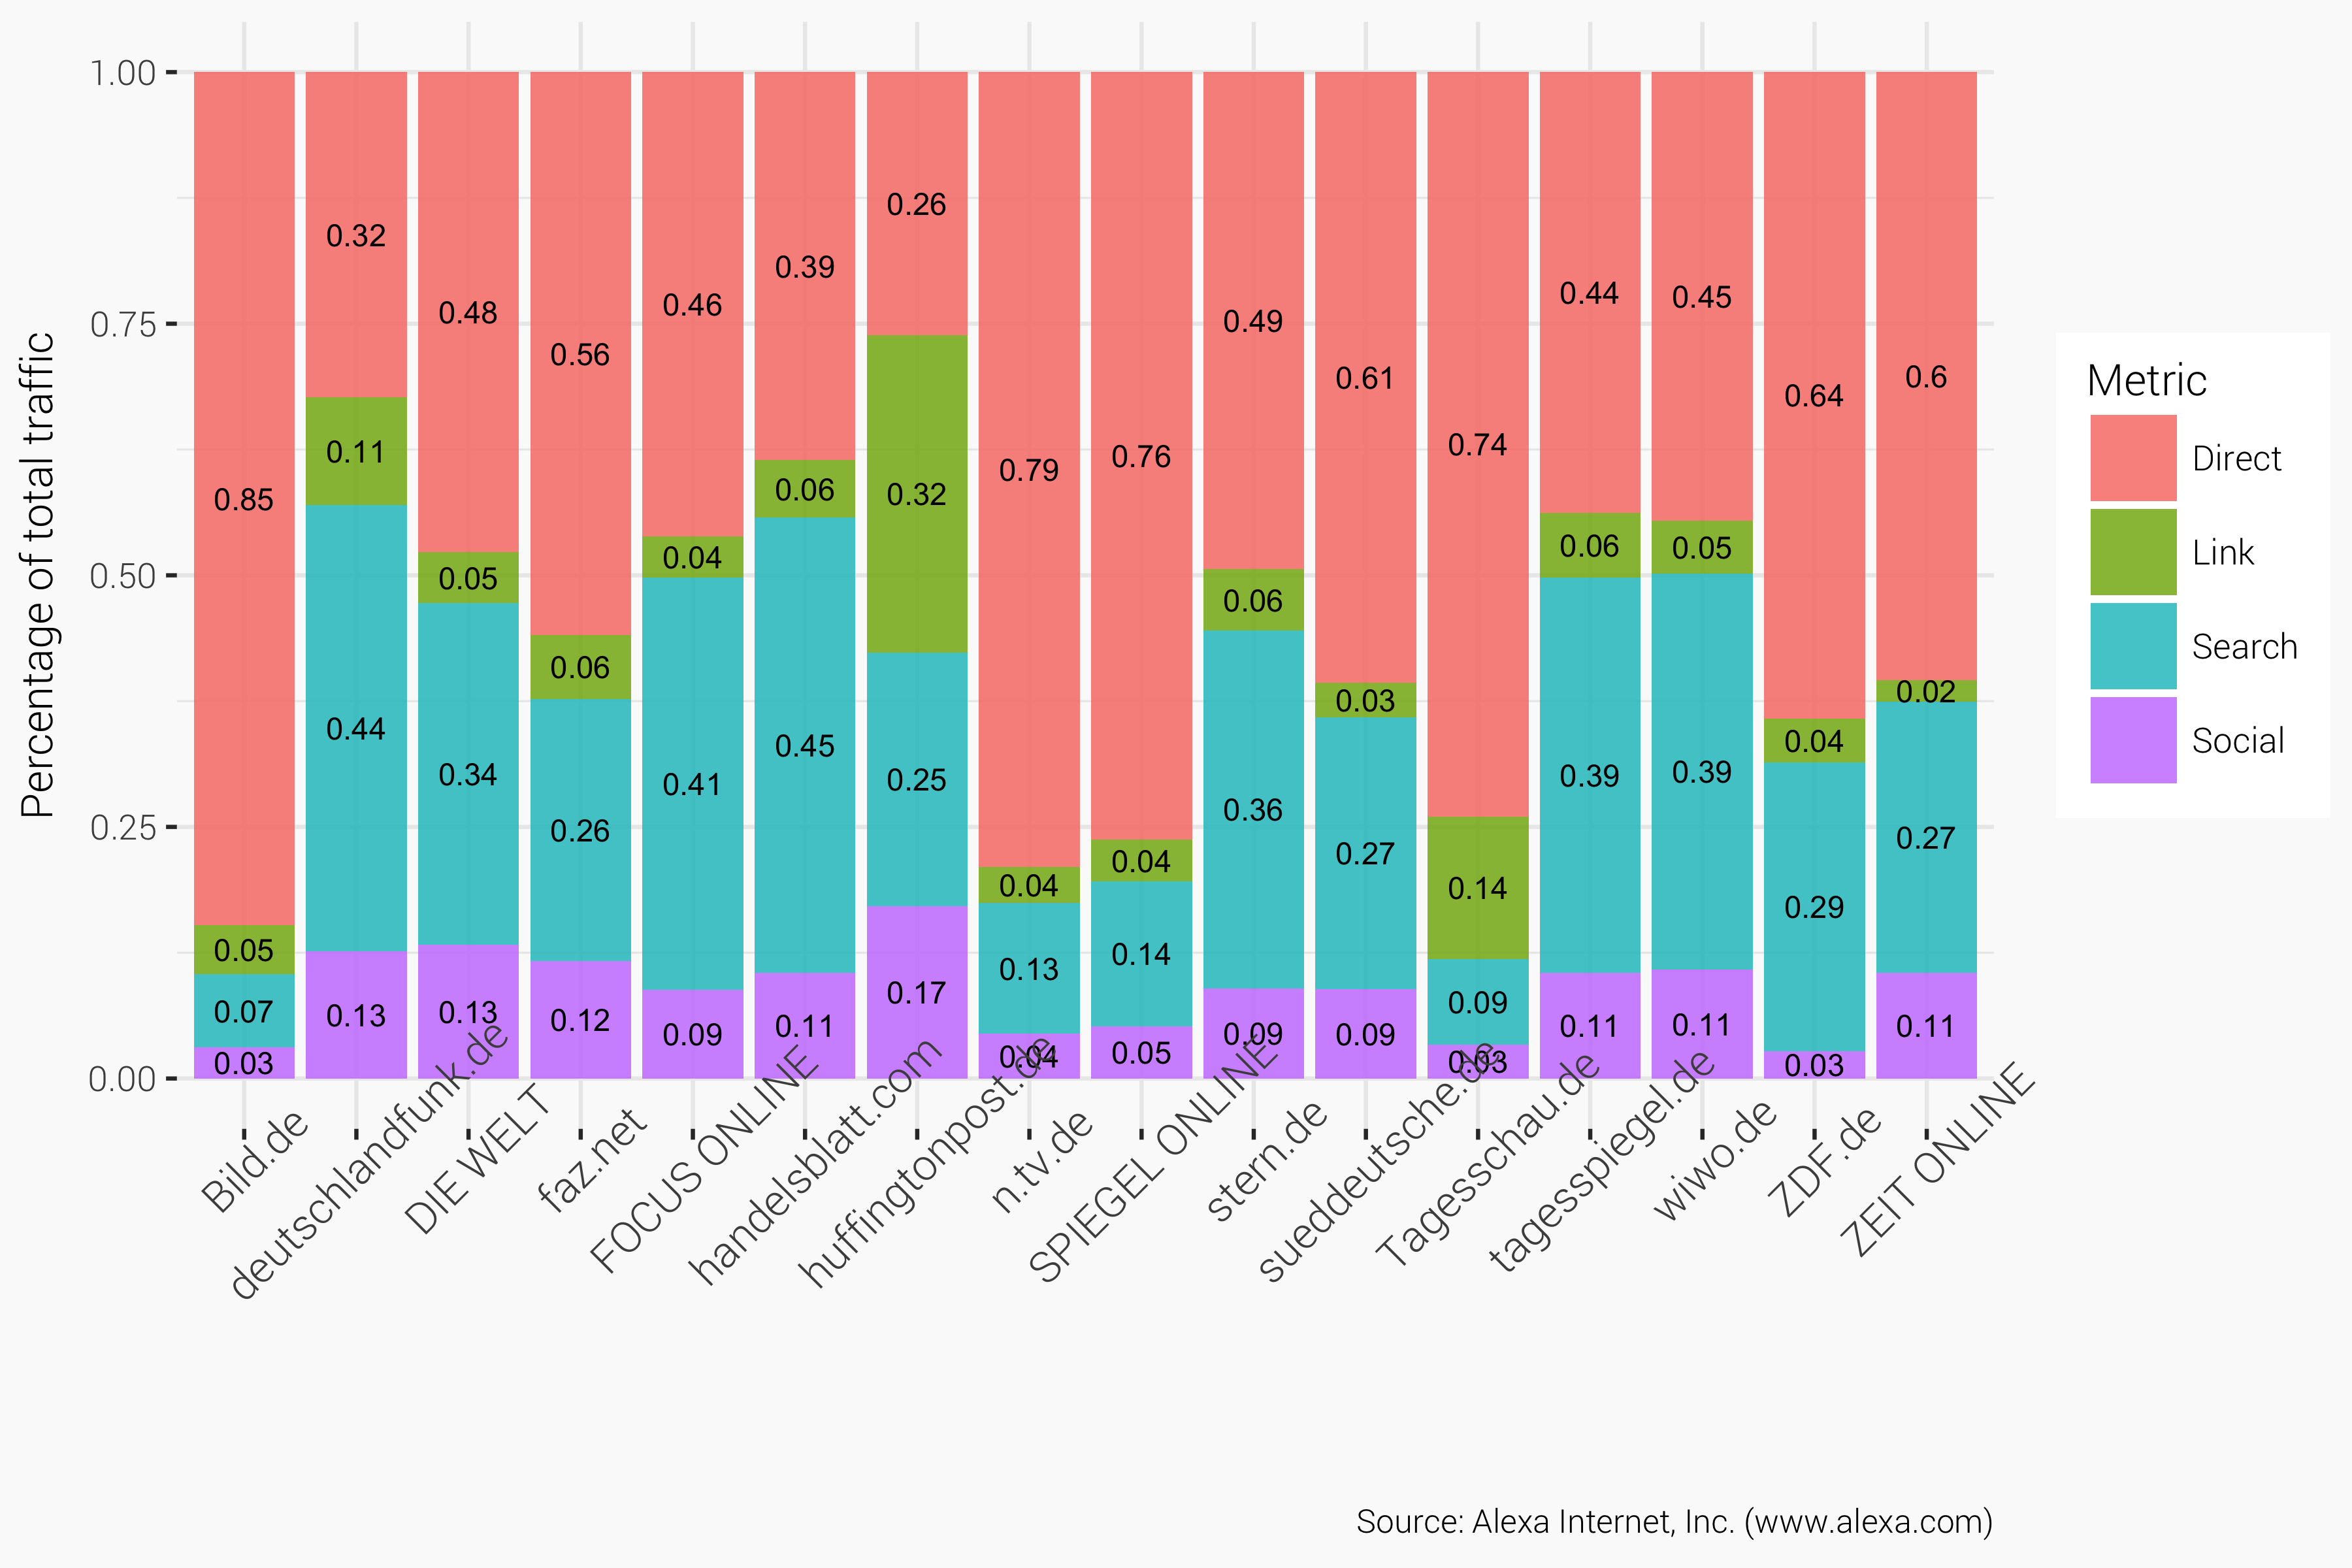
\includegraphics[width=0.8\textwidth]{../figs/traffic_source.png}
		\label{fig_traffic}
	\end{center}
\end{figure}

\begin{figure}[H]
	\caption{Search traffic \%}
	\begin{center}
		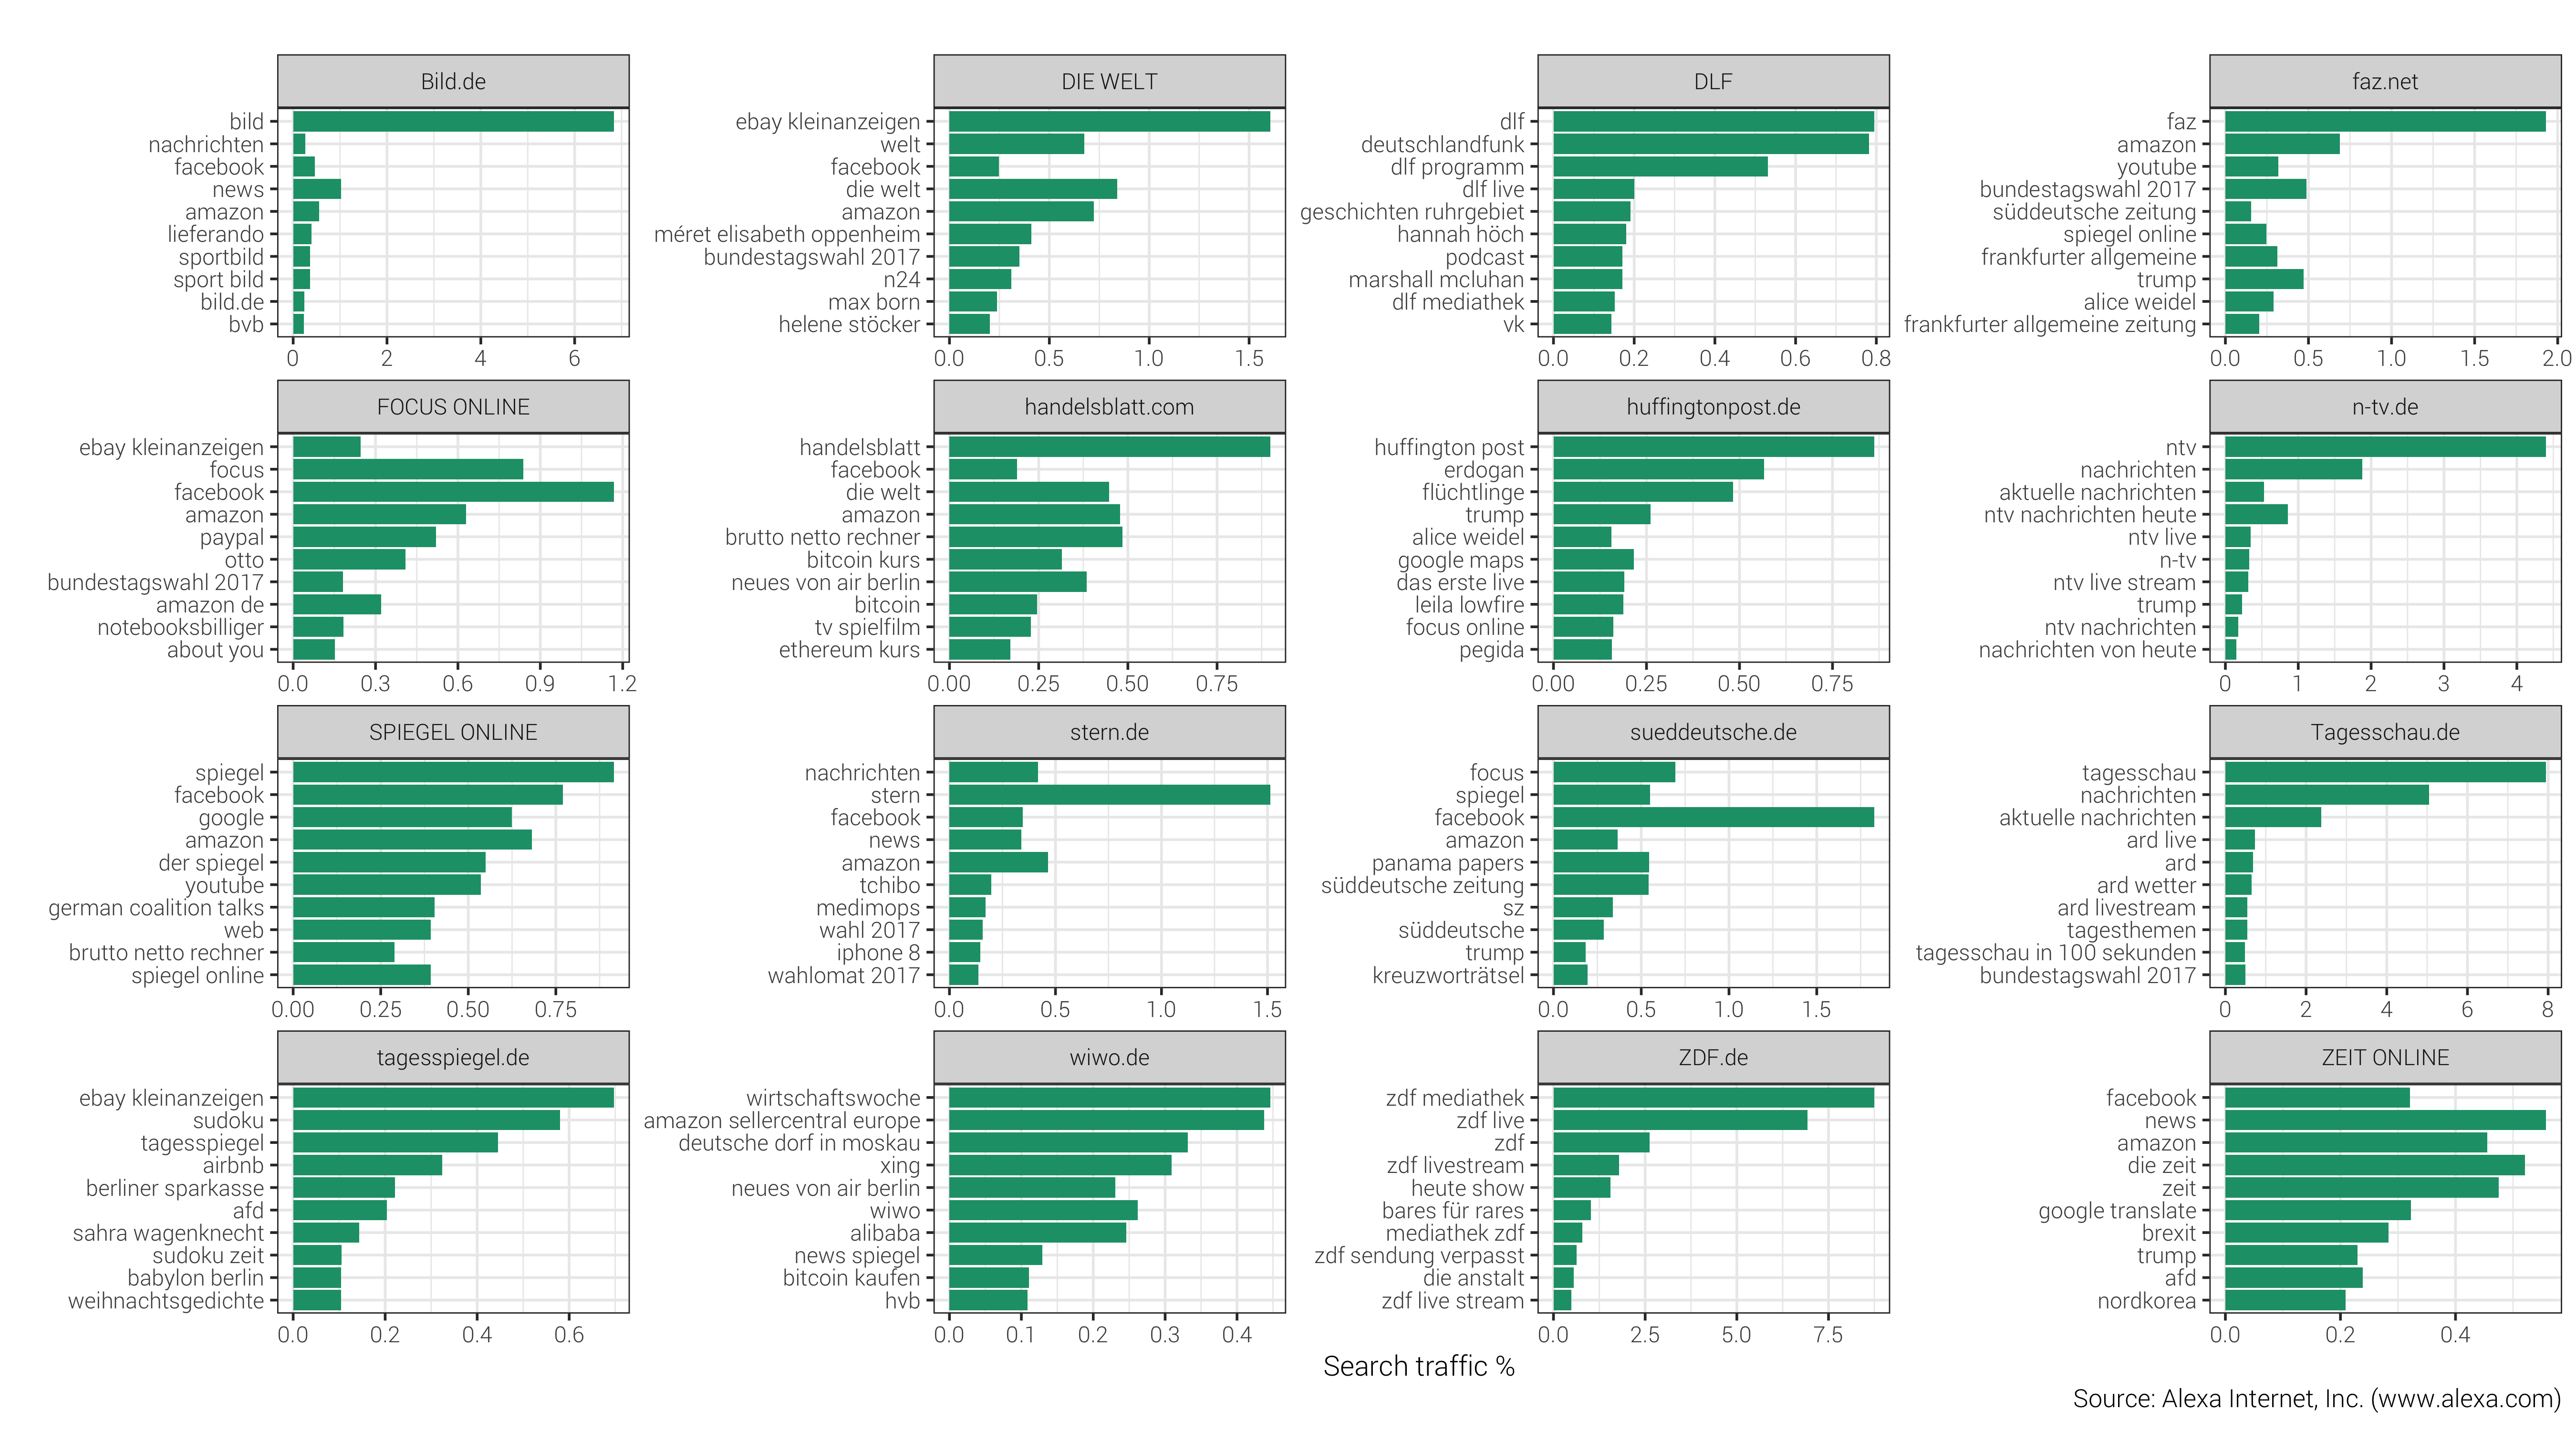
\includegraphics[width=0.8\textwidth]{../figs/search_traffic.png}
		\label{fig_searchtraffic}
	\end{center}
\end{figure}

Assuming that each search query is in itself a market where providers compete for traffic, the share of search queries for a keyword that has led visitors to a news page is the market share of that provider. In this context, figures \ref{fig_keywords1} and \ref{fig_keywords2} show the market share of providers for different keywords.\footnote{The figures show the percentage of searches for a keyword that sent traffic to a website in major search engines over the time span Jun-Dec 2017.} Nearly 15\% of all search queries for the keyword "Bundestagswahl 2017" (federal elections 2017) were forwarded to DIE WELT. FOCUS ONLINE, faz.net and SPIEGEL ONLINE obtained a market share of 7\% - 8\%. For the keyword "Groko" (grand coalition between CDU/CSU and SPD), SPIEGEL ONLINE was able to gain the largest market share (17\%) in the past six months, followed by DIE WELT (\%10), FOCUS ONLINE (8\%) and Bild.de (7.5\%). Figure \ref{fig_keywords2} shows the market share of news pages for the keyword search for a specific party. 

Contrary to figure \ref{fig_keywords1} , the x-axes in figure \ref{fig_keywords2} are scaled equally to show not only the market share of news sites for a specific party-keyword, but also for which party this provider has the largest market share. For example, we can see that the market share of sueddeutsche.de is largest for the keyword "Die Grünen". However, the biggest market share among the listed news providers for this keyword has Zeit.de. The largest market share for the keyword "AfD" can be found at DIE WELT, followed by SPIEGEL ONLINE. The proportion of public news providers is comparatively low for all keywords. 

\begin{figure}[H]
	\begin{center}
			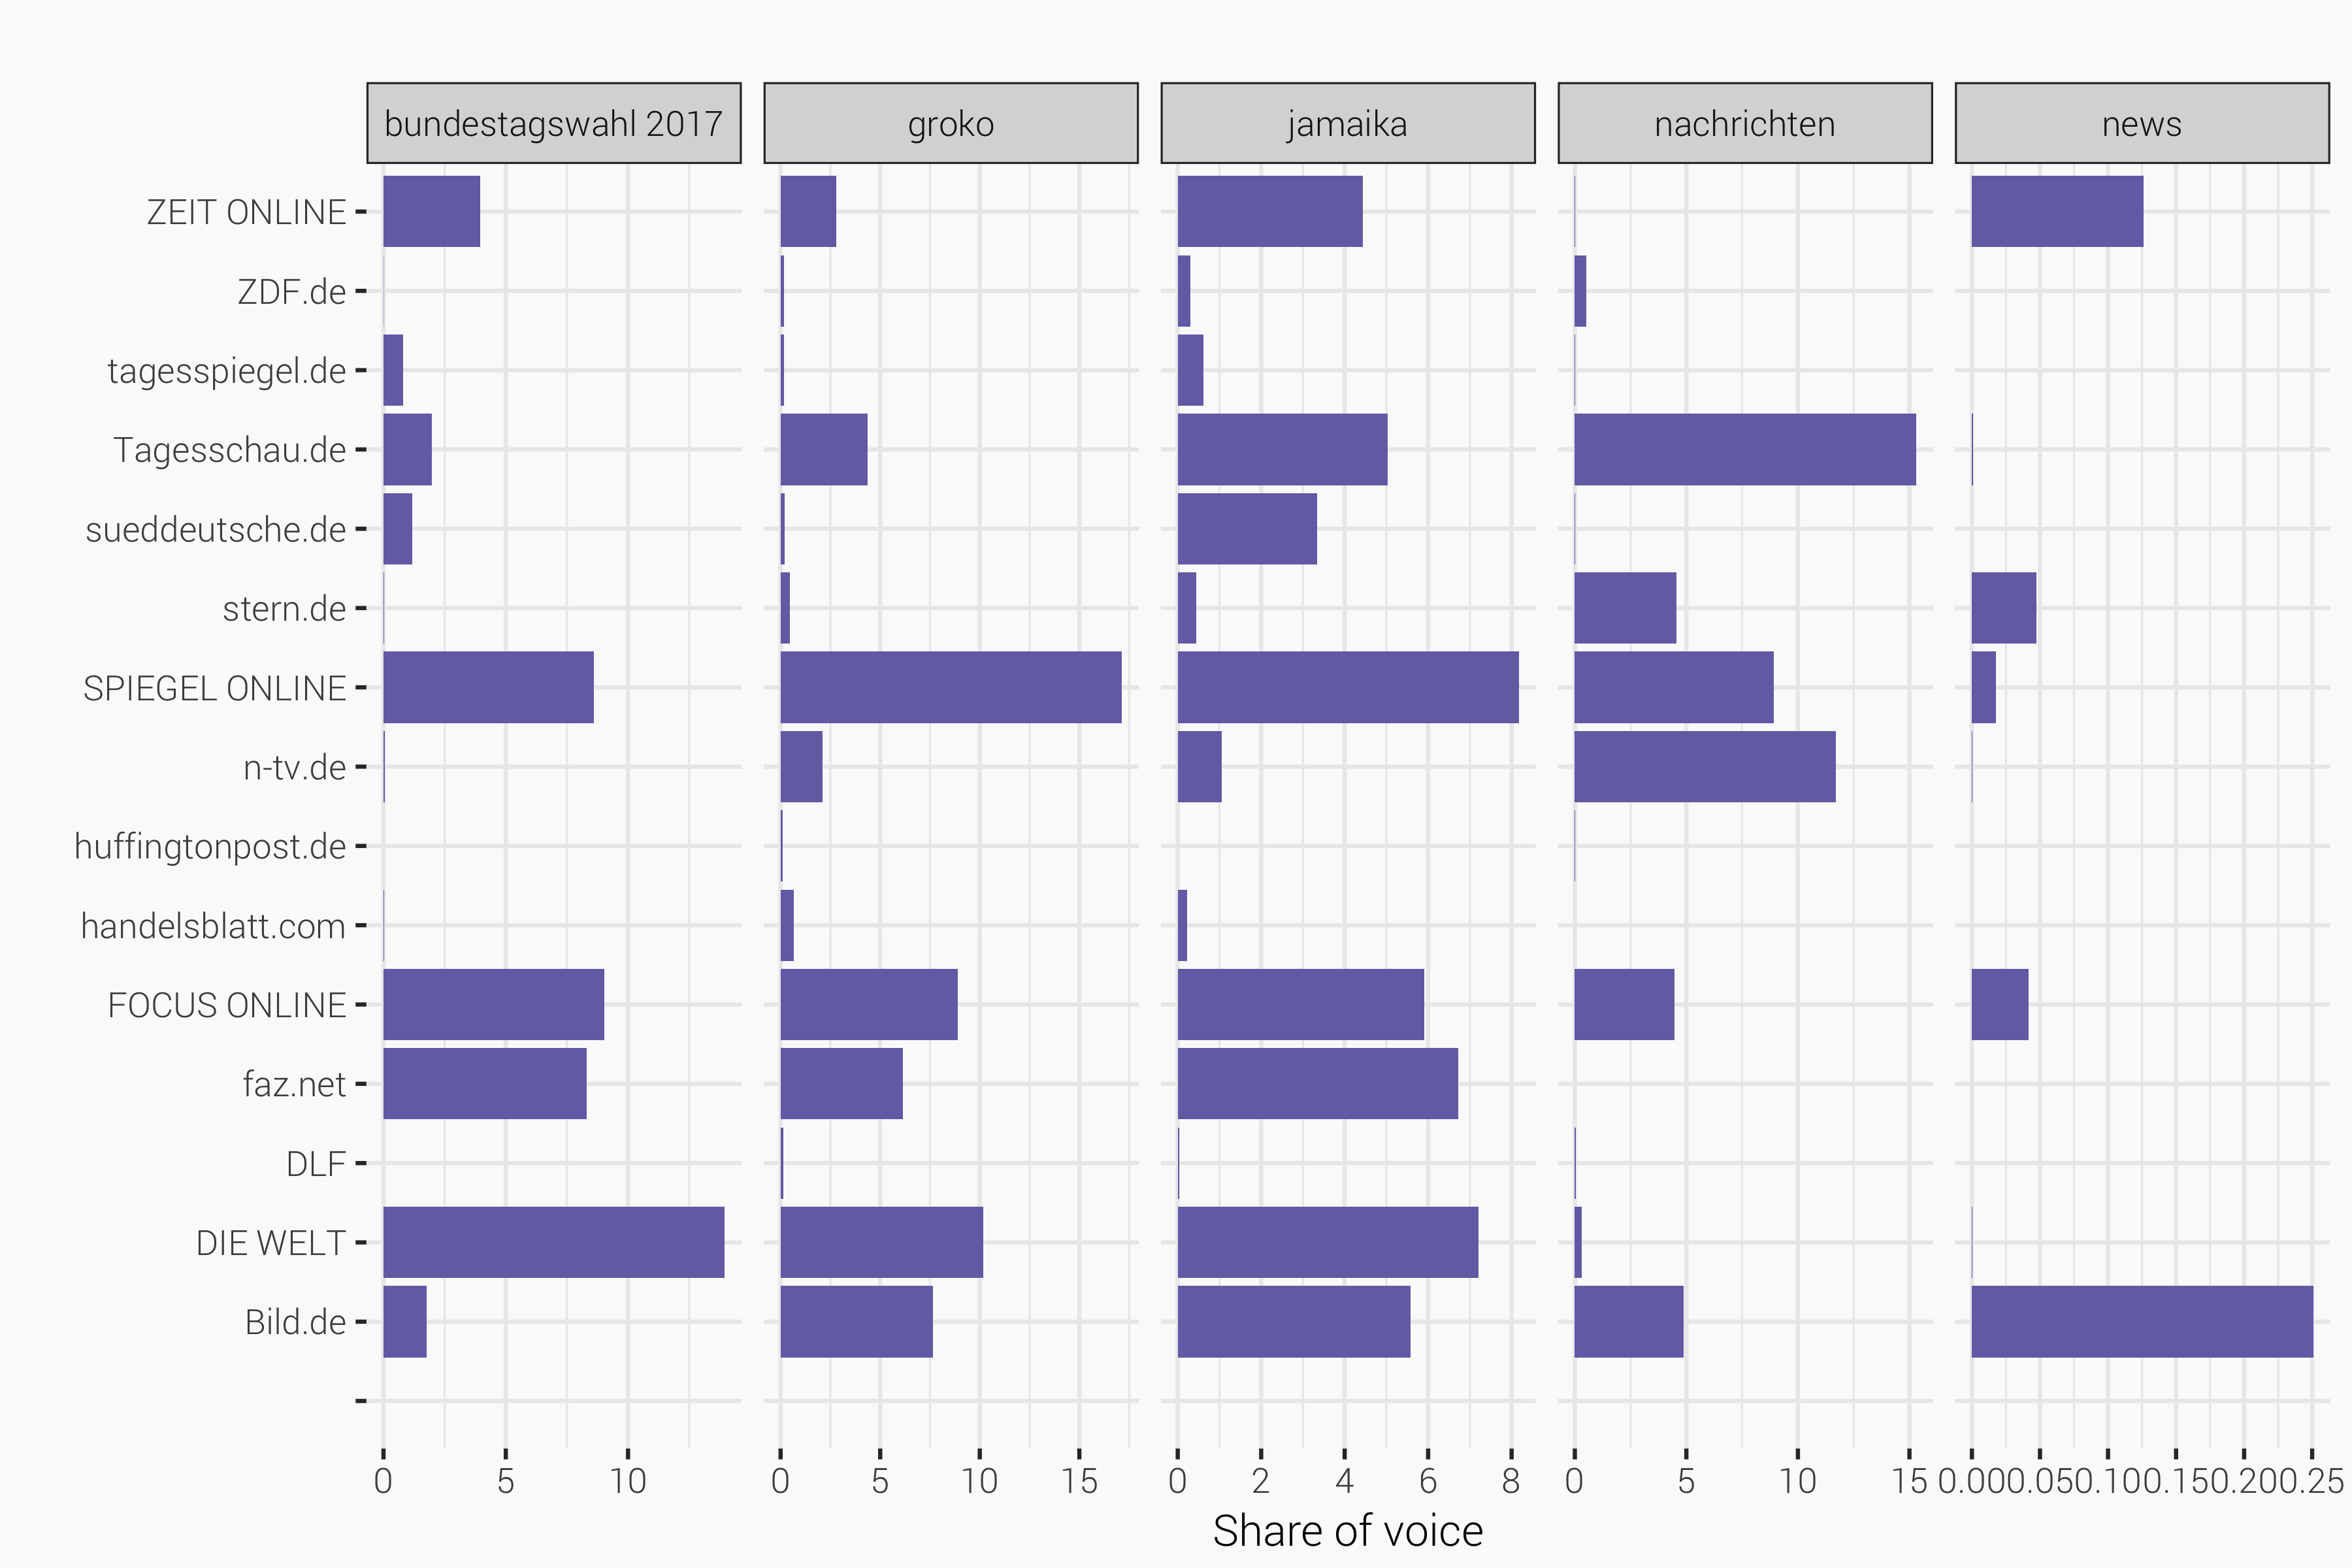
\includegraphics[width=.8\textwidth]{../figs/keywords1.png}
			\caption{Keyword market share for policy topics / general}
			\label{fig_keywords1}
	\end{center}
\end{figure}

\begin{figure}[H]
	\begin{center}
			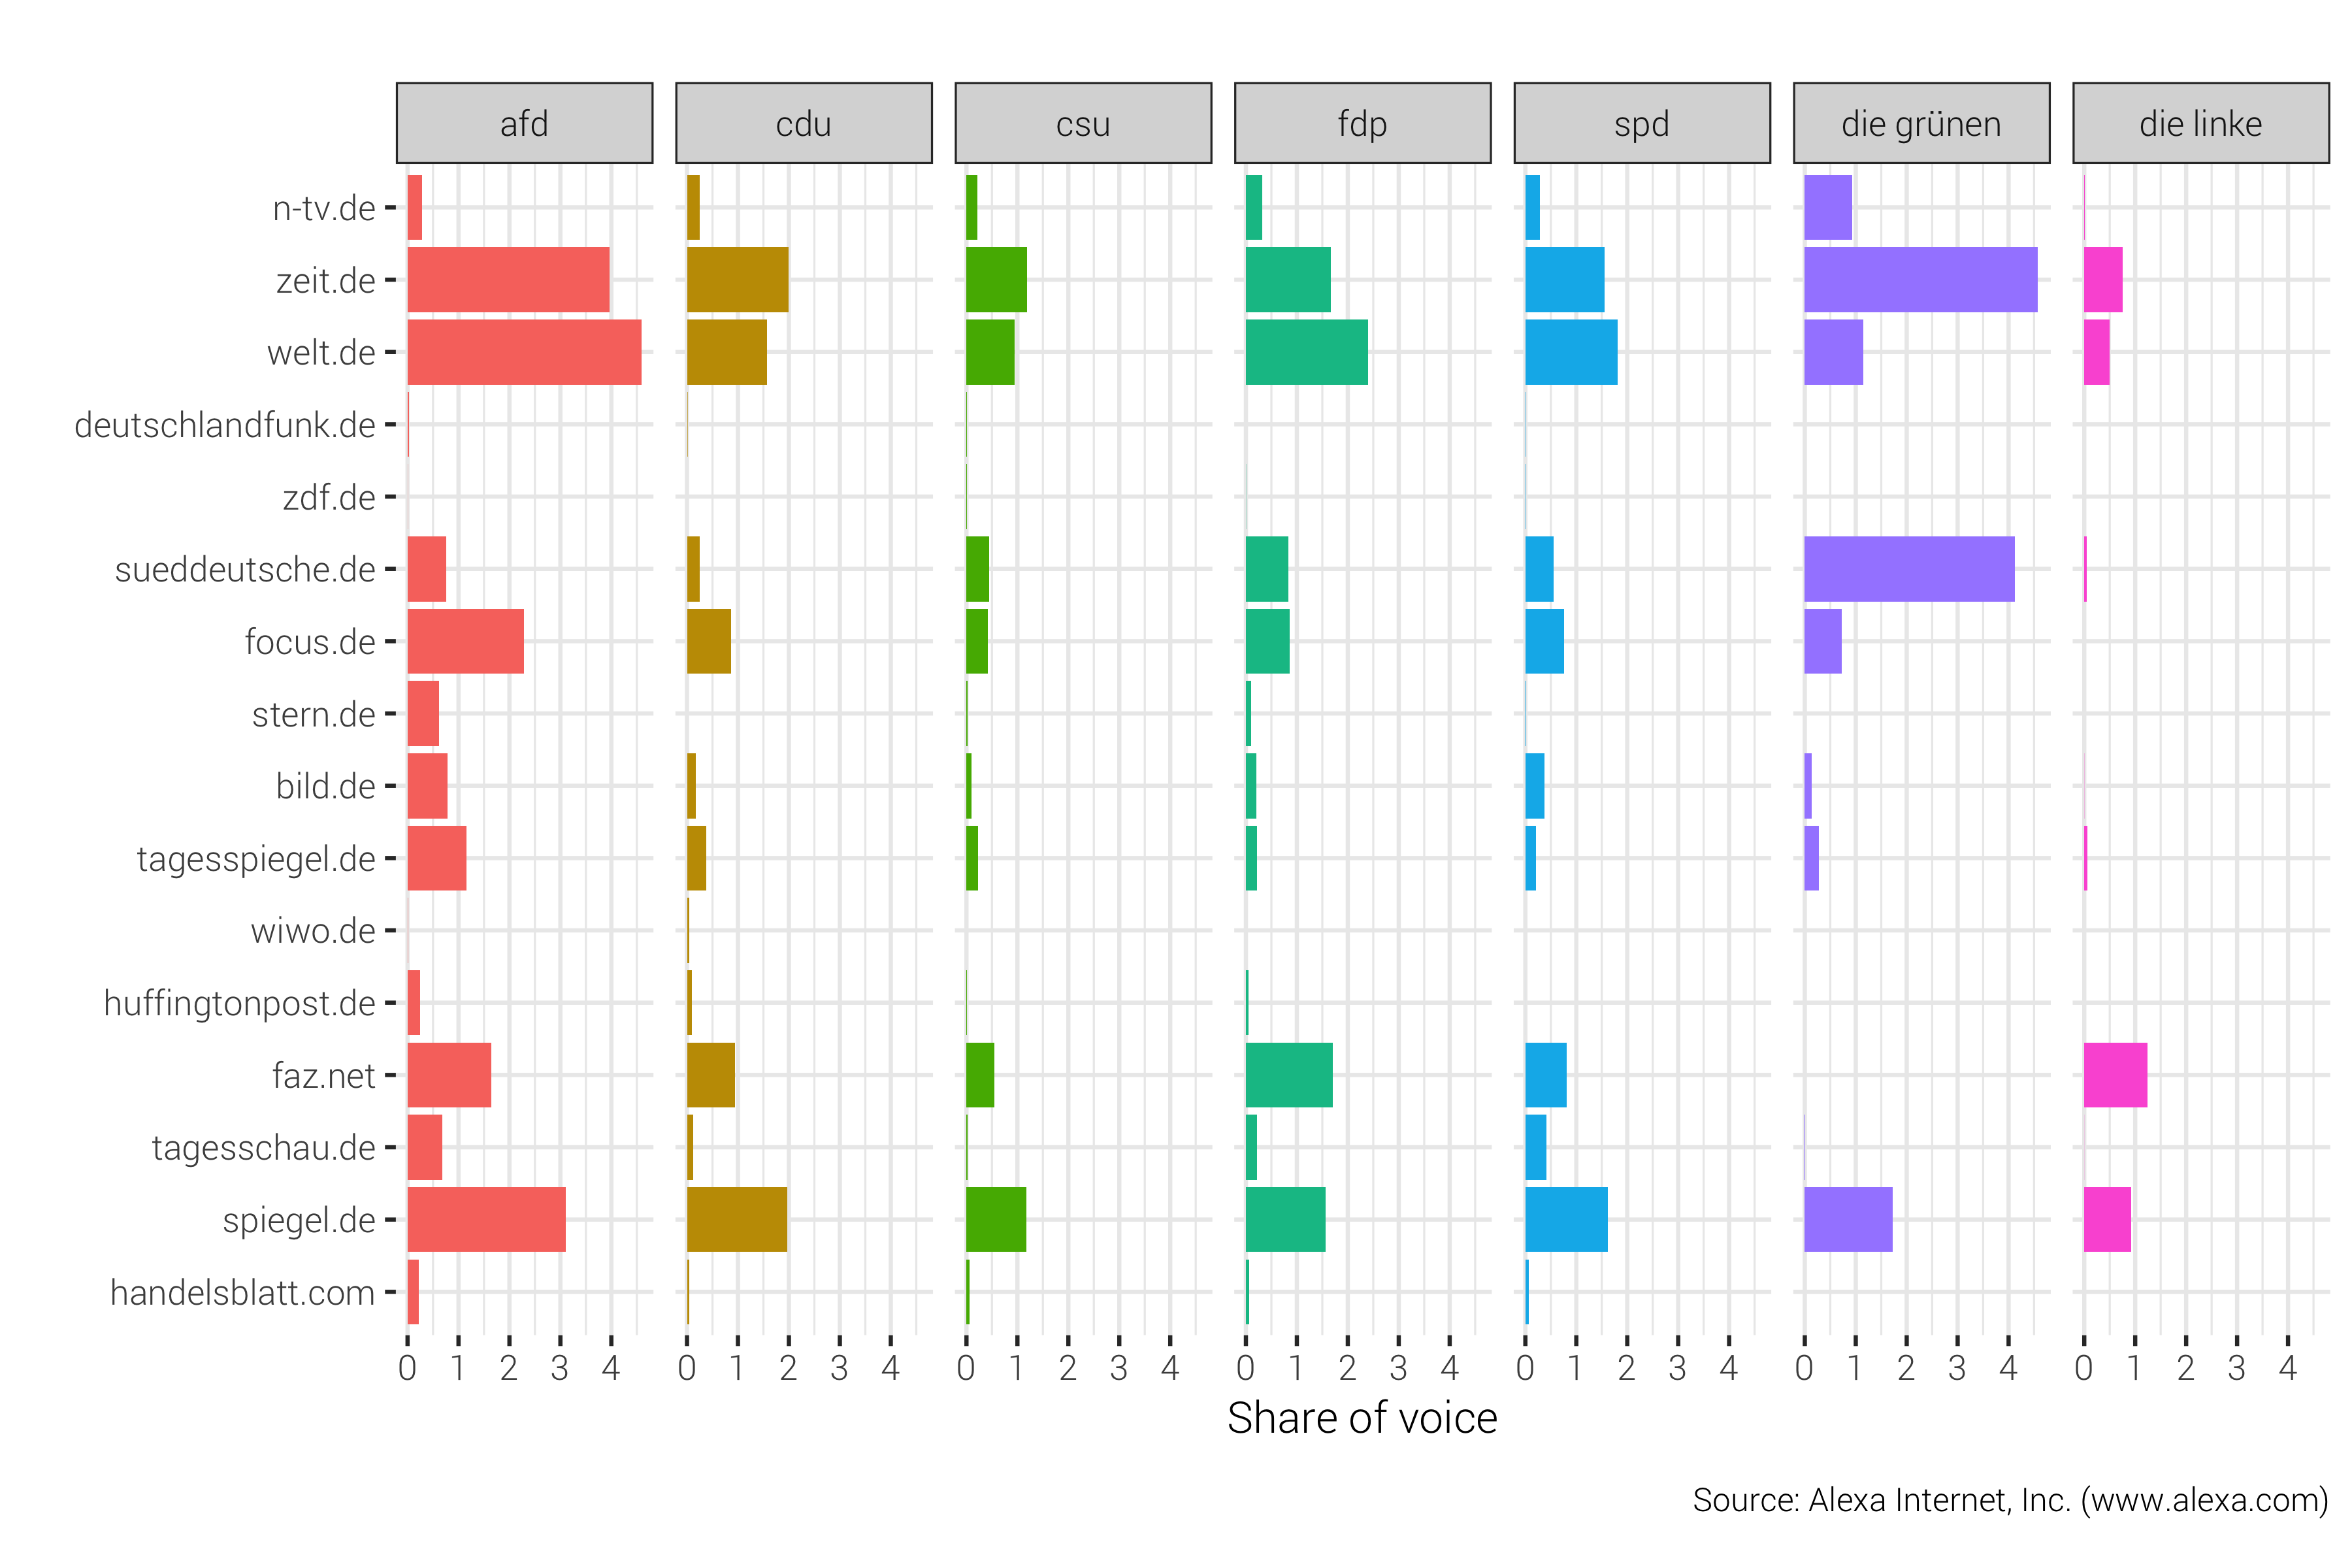
\includegraphics[width=.8\textwidth]{../figs/keywords2.png}
			\caption{Keyword market share for party-keywords}
			\label{fig_keywords2}
	\end{center}
\end{figure}


\section{Related Literature}

% Quantitative approaches
% -----------------------

Facebook is an important traffic supplier for news sites: Over 487.000 news articles from TOP15\footnote{Bild.de, bunte, Chip, FAZ, Focus, Handelsblatt, Heise, N-TV, Spiegel, Sport1, Stern, Süddeutsche, Tagesschau, Welt, Zeit} media were shared 123.000.000 times on Facebook (94\%), Twitter(3.5\%) and Google+(2.3\%).\cite{schiller_development_2016} In addition to the quantity of the audience, the demographic characteristics of recipients also have an influence on the willingness to pay on the advertiser site. Online advertising makes it possible to target ads to particular consumers in real time. Facebook instant articles facilitates this targeting, as they make the public users profile data available to the publisher. However, not all topics are equally often distributed in social media.

% Politics and Newspaper
% ----------------------

In \citet{tetlock_giving_2007}, $c_i$ is a bag-of-words representation and the outcome of interest $v_i$ is the latent “sentiment” of Wall Street Journal columns, defined along a number of dimensions such as “positive,” “optimistic,” and so on. The author defines the function $f (\cdot)$ using a dictionary called the General Inquirer, which provides lists of words associated with each of these sentiment categories.2 The elements of $f(c_i)$ are defined to be the sum of the counts of words in each category.

% Topic Modeling / LDA
% ---------------------------

Topic modeling is a statistical and computational technique for discerning information about the contents of a large corpus of documents without reading or annotating the original texts. A topic model uncovers patterns of word co-occurrence across the corpus, yielding a set of word clusters, together with associated probabilities of occurrence, which constitute the topics.

See \citep{taddy_estimation_2012} for a review of topic estimation techniques)

Since its introduction into text analysis, topic modeling has become hugely popular.8 (See \citet{blei_probabilistic_2012} for an overview.) The model has been especially useful in political science (e.g., \citep{grimmer_bayesian_2010}), where researchers have been successful in attaching political issues and beliefs to the estimated latent topics.

Topic modeling is alternatively labeled as “latent Dirichlet allocation,” (LDA) which refers to the Bayesian model in \citet{blei_latent_2003} that treats each $\boldsymbol{v}_i$ and $\boldsymbol{\theta}_l$ as generated from a Dirichlet - distributed prior.
The same model was independently introduced in genetics by \citet{pritchard_inference_2000} for factorizing gene expression as a function of latent populations; it has been similarly successful in that field. 

The basic topic model has been generalized and extended in variety of ways. A prominent example is the dynamic topic model of \citet{blei_dynamic_2006}, which considers documents that are indexed by date (e.g., publication date for academic articles) and allows the topics, say $\boldsymbol{\Theta}_t$, to evolve smoothly in time. 

% Structural topic models (STM)
% ----------------------------
A typical application of topic modeling in the social sciences first estimates LDA, then uses estimates of $\theta_d$ as the dependent variable in an regression on covariates to test whether different types of documents have different content. 

This is contradictory because documents are assumed to be generated by a statistical process that we subsequently reject.

The structural topic model (STM) of Roberts et. al. (2016) explicitly introduces covariates into a topic model, and allows one to estimate the impact of document-level covariates on topic content and prevalence as part of the topic model itself.

% ---------------------------------
% Statistical Analysis of Text Data
% ----------------------------------
\section{Statistical Analysis of Text Data}

Consider a collection of documents by $d \in \lbrace 1 ... D \rbrace$, each containing $n \in \lbrace 1 ... N_d \rbrace$ words. Primary observations consist of words $w_{d,n,}$ that are instances of unique terms from a vocabulary of terms, indexed by $v \in \lbrace 1 ... V \rbrace$. 

To use text as data and reduce the dimensionality, a common strategy is to (a) pre-process the text by imposing some preliminary restrictions (stop-word removal, tokenization) based on the nature of the data (twitter text, newspaper articles, speeches, etc.) and (b) to represent a document $d$ as a vector of word counts, $\boldsymbol{n}_d \in \boldsymbol{N}^V$. This representation is often referred to as the bag of words model, since the order in which words are used within a document is completely disregarded. Nowadays, the bag of words model is a common representation for most of statistic literature about text data analysis (\citet{blei_latent_2003}; \citet{erosheva_mixed-membership_2004}; \citet{griffiths_finding_2004}; \citet{genkin_large-scale_2007}).

Term-Document matrices represent frequency distribution of unique terms in the documents. Any one document will contain only a subset of all unique terms, and the rows corresponding to unused terms will all be zero.The key task then becomes how to extract low-dimensional information from documents that are high-dimensional by nature. This is analogous to a situation in which a researcher has a database with thousands of covariates and is attempting to choose which subset of them, or which summary statistics, should be included in regression analysis.
% The description of the data and how it was processed in order to reduce it to a manageable scale without losing significant information can be found in chapter ... 

We used the URL of these articles, to check how many times they where shared on Facebook using the \textit{sharedcount} API.\footnote{http://docs.sharedcount.com/} The returned share count is the sum of (1) the number of likes of this URL, (2) the number of shares of this URL (including copy-pasting a link back to Facebook), (3) the number of likes and comments on stories on Facebook about this URL and (4) the number of inbox messages containing this URL as an attachment.\footnote{See https://developers.facebook.com/docs/graph-api for more information about the Facebook Graph API.}

\begin{enumerate}
	\item Represent raw text $D$ as a numerical array $\boldsymbol{C}$. 
	 
	\item Map $\boldsymbol{C}$ to predict values $\boldsymbol{\hat{V}}$ of unknown outcomes $\boldsymbol{V}$. 
	
	E.g. the variable of interest $\boldsymbol{V}$ is an indicator whether the email is spam. The prediction $\boldsymbol{\hat{V}}$ determines whether or not to send the email to a spam filter. Sometimes the attribute of interest is latent, such as the topics of a newspaper article.
	\item Use $\boldsymbol{\hat{V}}$ in subsequent descriptive or causal analysis.
\end{enumerate}


Regarding 2, the methods to connect counts $\boldsymbol{c}_i$ to attributes $\boldsymbol{v}_i$ can be roughly divided into four categories \citep{gentzkow_text_2017}:
\begin{enumerate}
	\item Dictionary-based methods: 
	No statistical inference. Simply specify $\boldsymbol{\hat{v}_i}=f(\boldsymbol{c}_i)$ for some unknown function $f(\cdot)$. Sometimes based on a specific dictionary of terms (\citet{tetlock_giving_2007}, \citet{baker_measuring_2015}).
	\item Text regression methods:
	Directly estimate the conditional outcome distribution $p(\boldsymbol{v}_i|\boldsymbol{c}_i)$. Intuition: If we want to predict $\boldsymbol{v_i}$ from $\boldsymbol{c}_i$, we would regress the observed values of the former ($\boldsymbol{V}^{train}$) on the corresponding latter ($\boldsymbol{C}^{train}$). High dimensionality of $\boldsymbol{c}_i$ ($p > n^{train}$) requires use of appropriate regression techniques to avoid overfitting (e.g. $L_1$ regularized linear or logistic regression)
	\item Generative model of $p(\boldsymbol{c}_i|\boldsymbol{v}_i)$.
	Intuition: In many cases the underlying causal relationship runs from outcomes to language rather than the other way around. E.g. Google searches about flu do not cause flu cases to occur, rather, people with flu are more likely to produce such searches.
	\begin{enumerate}
		\item Observed attributes (supervised methods):
		Supervised machine learning starts with a researcher classifying observations to ‘train’ an algorithm under human ‘supervision’ – to ‘learn’ the correlation between the researcher’s ascribed classes and words characteristic of documents in those classes (Grimmer and Stewart (2013)). Fitting the model based on the observed training data $\boldsymbol{V}^{train}$, say $f_{\boldsymbol{\theta}}(\boldsymbol{c}_i;\boldsymbol{v}_i)$ for a vector of parameters $\boldsymbol{\theta}$, to this training set. The fitted model $f_{\hat{\boldsymbol{\theta}}}$ can be inverted in order to infer $\boldsymbol{v}_i$ for documents in the test set.
		\item Latent attributes (unsupervised methods): The function relating $\boldsymbol{c}_i$ to $\boldsymbol{v}_i$ is unknown, as we cannot observe the true value of $v_i$. Principal component analysis (PCA), latent Dirichlet allocation (LDA, topic modeling, structural-topic modeling). Unsupervised machine learning involves taking unclassified observations and uncovering hidden patterns that structure them in some meaningful way. The outputs of algorithms for unsupervised machine learning can be used as inputs into econometric models for predicting some variable of interest, but this is a different approach from intentionally choosing the dimensions of content based on their predictive ability.
	\end{enumerate}
	\item Deep learning techniques: neural networks, distributed language models.
\end{enumerate}

The goal of this paper is to find the latent topics within newspaper articles and how different types of media outlets (as well as the date?) influence the topic prevalence as well as the language to describe a topic (the word-topic distribution). We implement generative model (topic model). 
% A description of the generative process can be found in chapter ...

% ----------------------
% the online news market
% ----------------------
\section{The online news market}\label{ch_onlinenews}
% Kapitel raus? Bzw. mit Kapitel 4 zusammenlegen. 

The market for media content in Germany is characterized by the coexistence of public and private broadcasters. By shifting media content to the Internet, the dual system, which has been shaping the German television and radio landscape since the introduction of private broadcasting in the early 1980s, is facing a radical change. Since 2000, public broadcasting has expanded its range of services, particularly in the digital media sector. In 2017, 22 own websites and 100 apps were operated by public broadcasters on which they offer their content. As a result, public broadcasting no longer only competes with private television and radio stations, but also enters the market for online news. In the following, the characteristics of the market for online news in Germany are briefly described. 

Private media outlets naturally appear as two-sided platforms, that allow interaction between two categories of consumers: audiences and advertisers. As the demand on both consumer-sides are linked via indirect network externalities, the market in which media outlets operate are referred to as two-sided or multi-sided markets. The theoretical literature on two-sided markets originates from the analysis of credit card markets \citep{rochet_platform_2003} and was later transferred to the concept of other industries, such as dating agencies, real estate agents, and internet “business-to-business” websites \citep{caillaud_chicken_2003}. The basic concept of two-sided markets was already discussed decades ago in several economic studies, especially on media markets \citep{corden_maximisation_1952}, \citep{gustafsson_circulation_1978}, \citep{blair_pricing_1993}. However, comprehensive analyses have only been carried out in the last ten years, starting with the works of \citet{rochet_platform_2003}, \citet{evans_empirical_2003} and \citet{armstrong_competition_2006}.

Advertising-supported media such as online newspapers are typical examples of two-sided markets where the newspaper can be conceived as platforms that allow interaction between audiences ("eyeballs") and advertisers. The newspaper creates (or buys) content to attract viewers which in turn attract advertisers who pay for readers' attention \citep{evans_industrial_2005}. The size and characteristics of the audience has a positive effect on the advertisers' willingness to pay, as advertisements are typically sold based on cost per viewer, often expressed in terms of the cost of reaching a thousand viewers (CPM). Advertising can also have an effect on the recipients, which can be either negative or positive, depending on the quality of the advertising. Based on the strength of the indirect network effects, private publishers maximize their revenue by balancing the demand from advertisers and subscribers using different business models \citep{evans_economics_2008}. Many traditional newspapers follow the subscription/advertising model, where the publisher charges both market sides: The audience pays a fee to obtain access to the content, and advertisers pay to obtain access to the viewers. Many online news agencies provide part of their editorial content for free and hide another, more exclusive part behind a paywall. However, since the Internet has considerably simplified the possibilities for obtaining information and thus reduced the marginal utility of content, such a business model can only be efficient if the content behind the paywall is very exclusive. As a result, many publishers rely on a free-media model, in which the publishers do not charge viewers for access to the media at all, in order to attract as many eyeballs as possible to their platform, and thus, exploit the indirect network effects on the advertising site. In fact, most advertising-financed online magazines earn a large part of their gross margin from advertising \citep{evans_industrial_2005}. In order to maximize their profits, these companies have an interest in attracting as many readers as possible. In addition to the quantity of the audience, the demographic characteristics of recipients also have an influence on the willingness to pay on the advertiser site.
 
The two-sided market structure of the private news market results in news platforms striving to choose their content in such a way that its reach is as large as possible in order to maximize profits from advertising revenues. \citet{steiner_program_1952} concluded, that profit-maximizing media owners may choose to offer the same content, i.e. content aligned with the tastes of the majority. \citet{gabszewicz_press_2001} study the problem of diversity of the political content of newspapers. They find that the maximum differentiation only prevails if the readers sufficiently value the political differentiation between the newspapers the advertising market is small enough. On the other hand, advertising may also have a positive impact on the media, as it enables publishers to report independently of political parties. \citet{ellman_what_2009} analyze a theoretical framework of a two-sided market for newspaper, where readers value accuracy and advertisers value advert-receptive readers. They found that advertising increases the intensity of competition for readers and therefore raises accuracy of media coverage. However, in the monopolistic case, newspapers under-report news that sufficiently reduces advertiser profits. 

Given the crucial role of the media in shaping opinion and promoting democracy, pluralism of opinion and accuracy of information is a major concern of public authorities. Public broadcasting in Germany originated in the post-war period and has always had the task of providing the entire population with independent media. This media offer is intended to guarantee diversity of opinion within the media landscape and to be economically and politically independent. The former is given by the fact that the public media are financed by compulsory fees. To take into account the distinct nature of digital media, the Interstate Broadcasting Agreement (Rundfunkstaatsvertrag) also regulates the scope for action of online services offered by public service broadcasting since 2007. Accordingly, public media are not allowed to distribute purchased content and must - depending on the category of content - set a time limit on its accessibility. In addition, there is a strict advertising ban and prohibition of regional reporting. 

The market for media content in Germany is characterized by the coexistence of public and private broadcasters. By shifting media content to the Internet, the dual system, which has been shaping the German television and radio landscape since the introduction of private broadcasting in the early 1980s, is facing a radical change. Since 2000, public broadcasting has expanded its range of services, particularly in the digital media sector. As a result, public broadcasting no longer only competes with private television and radio stations, but also enters the market for online news. 


\section{Generative Process}

In this unsupervised method, the words in a document are viewed as the realization of some stochastic process. The generative process is defined through a probability model for $p(\boldsymbol{c}_i|\boldsymbol{v}_i)$.

Each observation $\boldsymbol{c}_i$ is a conditionally independent draw from the vocabulary of possible tokens accodring to some document-specific token probability vector $\boldsymbol{q}_i=[q_{i1}...q_{ip}]'$. Conditioning on document length, $m_i=\sum_jc_{ij}$, this implies a multinomial distribution for the counts

\begin{equation}\label{eq_1}
	\boldsymbol{c}_i \sim \boldsymbol{MN}(\boldsymbol{q}_i,m_i). 
\end{equation}

Under the basic model in \ref{eq_1}, a connection between text and attributes is defined through the link function $\boldsymbol{q}_i=q(\boldsymbol{v}_i)$. 

\begin{equation}\label{eq_2}
	\boldsymbol{E} \bigg[\frac{\boldsymbol{c}_i}{m_i}\bigg]=\boldsymbol{q}_i =v_{i1}\boldsymbol{\theta}_1+v_{i2}\boldsymbol{\theta}_2+v_{ik}\boldsymbol{\theta}_k=\boldsymbol{\Theta v}_i
\end{equation}

where attributes $v_{il}$ are referred as topic wights, restricting $v_{il}\geq 0$ and $\sum^k_{l=1}v_{il}=1$, and each topic $\boldsymbol{\theta}_l$ is a probability vector over possible tokens: $\theta_{lj}\geq 0$ and $\sum^p_{j=1}\theta_{il}=1$. Each $\boldsymbol{v}_i$ and $\boldsymbol{\theta}_l$ is generated from a Dirichlet-distributed prior.

Latent Dirichlet allocation (LDA) is a particularly popular method for fitting a topic model. It treats each document as a mixture of topics, and each topic as a mixture of words. This allows documents to “overlap” each other in terms of content, rather than being separated into discrete groups, in a way that mirrors typical use of natural language. Formally speaking, each document has its own probability distribution over topics. Then, for each word in each document, a topic assignment is made and then, conditional on the assignment, a word from the corresponding topic. 

Estimation of topic models make use of some alternating inference for $\boldsymbol{V|\Theta}$ and $\boldsymbol{\Theta|V}$.

\begin{enumerate}
	\item Expectation-maximization algorithm (EM)
	Either maximize the likelihood implied by \ref{eq_1} and \ref{eq_2} or, after incorporating the usual Dirichlet priors on $\boldsymbol{v}_i$ and $\boldsymbol{\theta}_l$ \citep{taddy_estimation_2012} 
	\item Target full posterior distribution $p(\boldsymbol{\Theta,V|c}_i})$
\end{enumerate}

Choice of number of topics $k$ is often fairly arbitrary. In practice it is very common to simply start with a number of topics on the order of ten, and then adjust the number of topics in whatever direction seems to improve interpretability. Whether this ad hoc procedure is problematic depends on the application. In many applications of topic models to date the goal is to provide an intuitive description of text rather than inference on some underlying “true” parameters; in these cases, the ad hoc selection of the number of topics may be reasonable.

Data-driven approaches: 
\begin{enumerate}
	\item \citet{taddy_estimation_2012} describes a model selection process for $k$ that is based upon Bayes factors.
	\item \citet{airoldi_reconceptualizing_2010} provide a cross-validation (CV) scheme
	\item \citet{teh_hierarchical_2006} use Bayesian nonparametric techniques that view $k$ as an unknown model parameter.
\end{enumerate}


\subsection{Structural Topic Model}

The process for generating individual words is the same as for plain LDA conditional on the $\beta_k$ and $\pi_d$ terms. 

However both objects can depend on potentially different sets of document-level covariates. Each document has:
\begin{enumerate}
	\item Topic Prevalence. Attributes $r_d$ that affect the likelihood of discussing topic $k$. how much of a document is associated with a topic
	\item Topic Content. Attributes $r_d$ that affect the likelihood of discussing term $v$ overall, and of discussing it within topic $k$. the words used within a topic
\end{enumerate}

The generation of the $k$ and $d$ terms is via multinomial logistic regression, which breaks local conjugacy.

The standard topic modeling technique, Latent Dirichlet Allocation (LDA), may have limited utility in the realm of social media. LDA makes a statistical assumption that all texts in the modeled corpus are generated by the same underlying process (Blei). Thus, it is not ideally suited to examining differences in topical content that are affected by external variables such as author identity or time of writing.

Structural topic modeling (STM) is a recently introduced variant of LDA that is designed to address precisely this limitation . STM can represent the effect of external variables on both topical content and topical prevalence. The external variables can consist of any metadata that distinguishes one text from another, including variables relating to author identity (gender, age, political affiliation, etc.), textual genre (for example, news stories versus academic articles), and time of production.

stmVigenette: "The goal of the Structural Topic Model is to allow researchers to discover topics and estimate their relationship to document metadata. Outputs of the model can be used to conduct hypothesis testing about these relationships."  

\subsubsection{Estimation of the STM}
In STM, metadata can be entered in the topic model in two ways: topical prevalence and topical content. Metadata covariates for topical prevalence allow the observed metadata to affect the frequency with which a topic is discussed. Covariates in topical content allow the observed metadata to affect the word rate use within a given topic{that is, how a particular topic is discussed.

We use the online magazine-type as a covariate in the topic prevalence portion of the model with the  data described above. Each document is modeled as a mixture of multiple topics. Topical prevalence captures how much each topic contributes to a document. Because different documents come from different sources, it is natural then to want to allow this prevalence to vary with metadata that we have about document sources.

We will simply let prevalence be a function of the magazine variable, which is coded as either
Spiegel Online or FOCUS Online and the variable day which is an integer measure of days running from 01-01-2017 to 31-07-2017.

\subsection{Gibbs Sampler}\label{section_gibbs}

Strategy for discovering topics  \cite{griffiths_finding_2004}
\begin{itemize}
	\item Considering the posterior distribution over the assignments of words to topics, $P(z|w)$. (and not explicitly representing $\phi$ or $\theta$ as parameters to be estimated)
	\item Examine this posterior distribution to obtain $\phi$ or $\theta$
\end{itemize}


After making assumptions about the parameters (number of topics $K$, prior distributions $\alpha$ and $\beta$), the procedure of Gibbs sampling is as follows:

\begin{enumerate}
	\item Go through each document and randomly assign each word in the document to one of $K$ topics, based on the prior distributions.
	\item For each document $d$, go through each word $w$ and compute:
	\begin{enumerate}
		\item The document-topic distribution $\theta = p(t|d)$
		\item The topic-term distribution $\phi = p(w|t)$
	\end{enumerate}
	\item Reassign word $w$ a new topic $t^*$, where we choose topic $t^*$ with probability $p(t^*|d)*p(w|t^*)$
\end{enumerate}

On repeating the last step a large number of times, the algorithm reaches a steady state where topic assignments are pretty good. These posterior distributions $\theta$ and $\phi$ are then used to determine the topic mixtures of each document.

\subsection{Validate accuracy}

\begin{itemize}
	\item Manual audits: cross checking some subset of the fitted values against the coding a human would produce by hand
	\item Inspection of fitted parameters
	\item Interpretation of fitted topics usually proceeds by ranking the tokens in each topic according to token probability.
\end{itemize}

Caution against the over-interpretation of unsupervised models: posterior distributions informing parameter estimates are highly multimodal, and multiple topic model runs can lead to multiple different interpretations. Add some supervision (\citet{airoldi_improving_2016}, \citet{gentzkow_text_2017})  

% ----------------------
% Model Results
% ----------------------
\section{Empirical Evaluation}\label{ch_empirical}

This section summarizes the results of the STM. Subsequently different measures to analyze the content differences between public and private ownership are applied according to the following approaches: (1) To address the question whether market imperfections exist in that sense, that some topics are not covered by private but by public news provider, I use the document-topic probability $\theta$, to estimate the conditional expectation of topic prevalence for given document characteristics (See section \ref{subsectiona_topicprevalence}). (2) Next, I find all edges between topics where they exhibit a positive correlation of $\theta$ above 0.1 to examine how topics are correlated differently for different covariate levels, indicating how topics are connected and framed differently between private and public media (see section \ref{subsection_topiccorrelation}). Approaches (1) and (2) have been used in \citep{roberts_model_2016}. However, we extend the analysis by (3) calculating the similarity of the word-topic distribution $\beta$ between the news provider using various distance measures, to identify which topics are discussed similar or differently (see section \ref{subsection_similarity}). 

\subsection{Topic correlations}\label{subsection_topiccorrelation}

Next, the topic correlation is calculated, indicating how topics are connected and framed in public and private media. In Figure \ref{fig_topic_correlations}, indicates all edges between topics where they exhibit a positive correlation above 0.1 \citep{roberts_model_2016}.


\begin{figure}[H]
	\caption{Topic Correlation}
		\begin{center}
		\begin{subfigure}{.7\textwidth}
			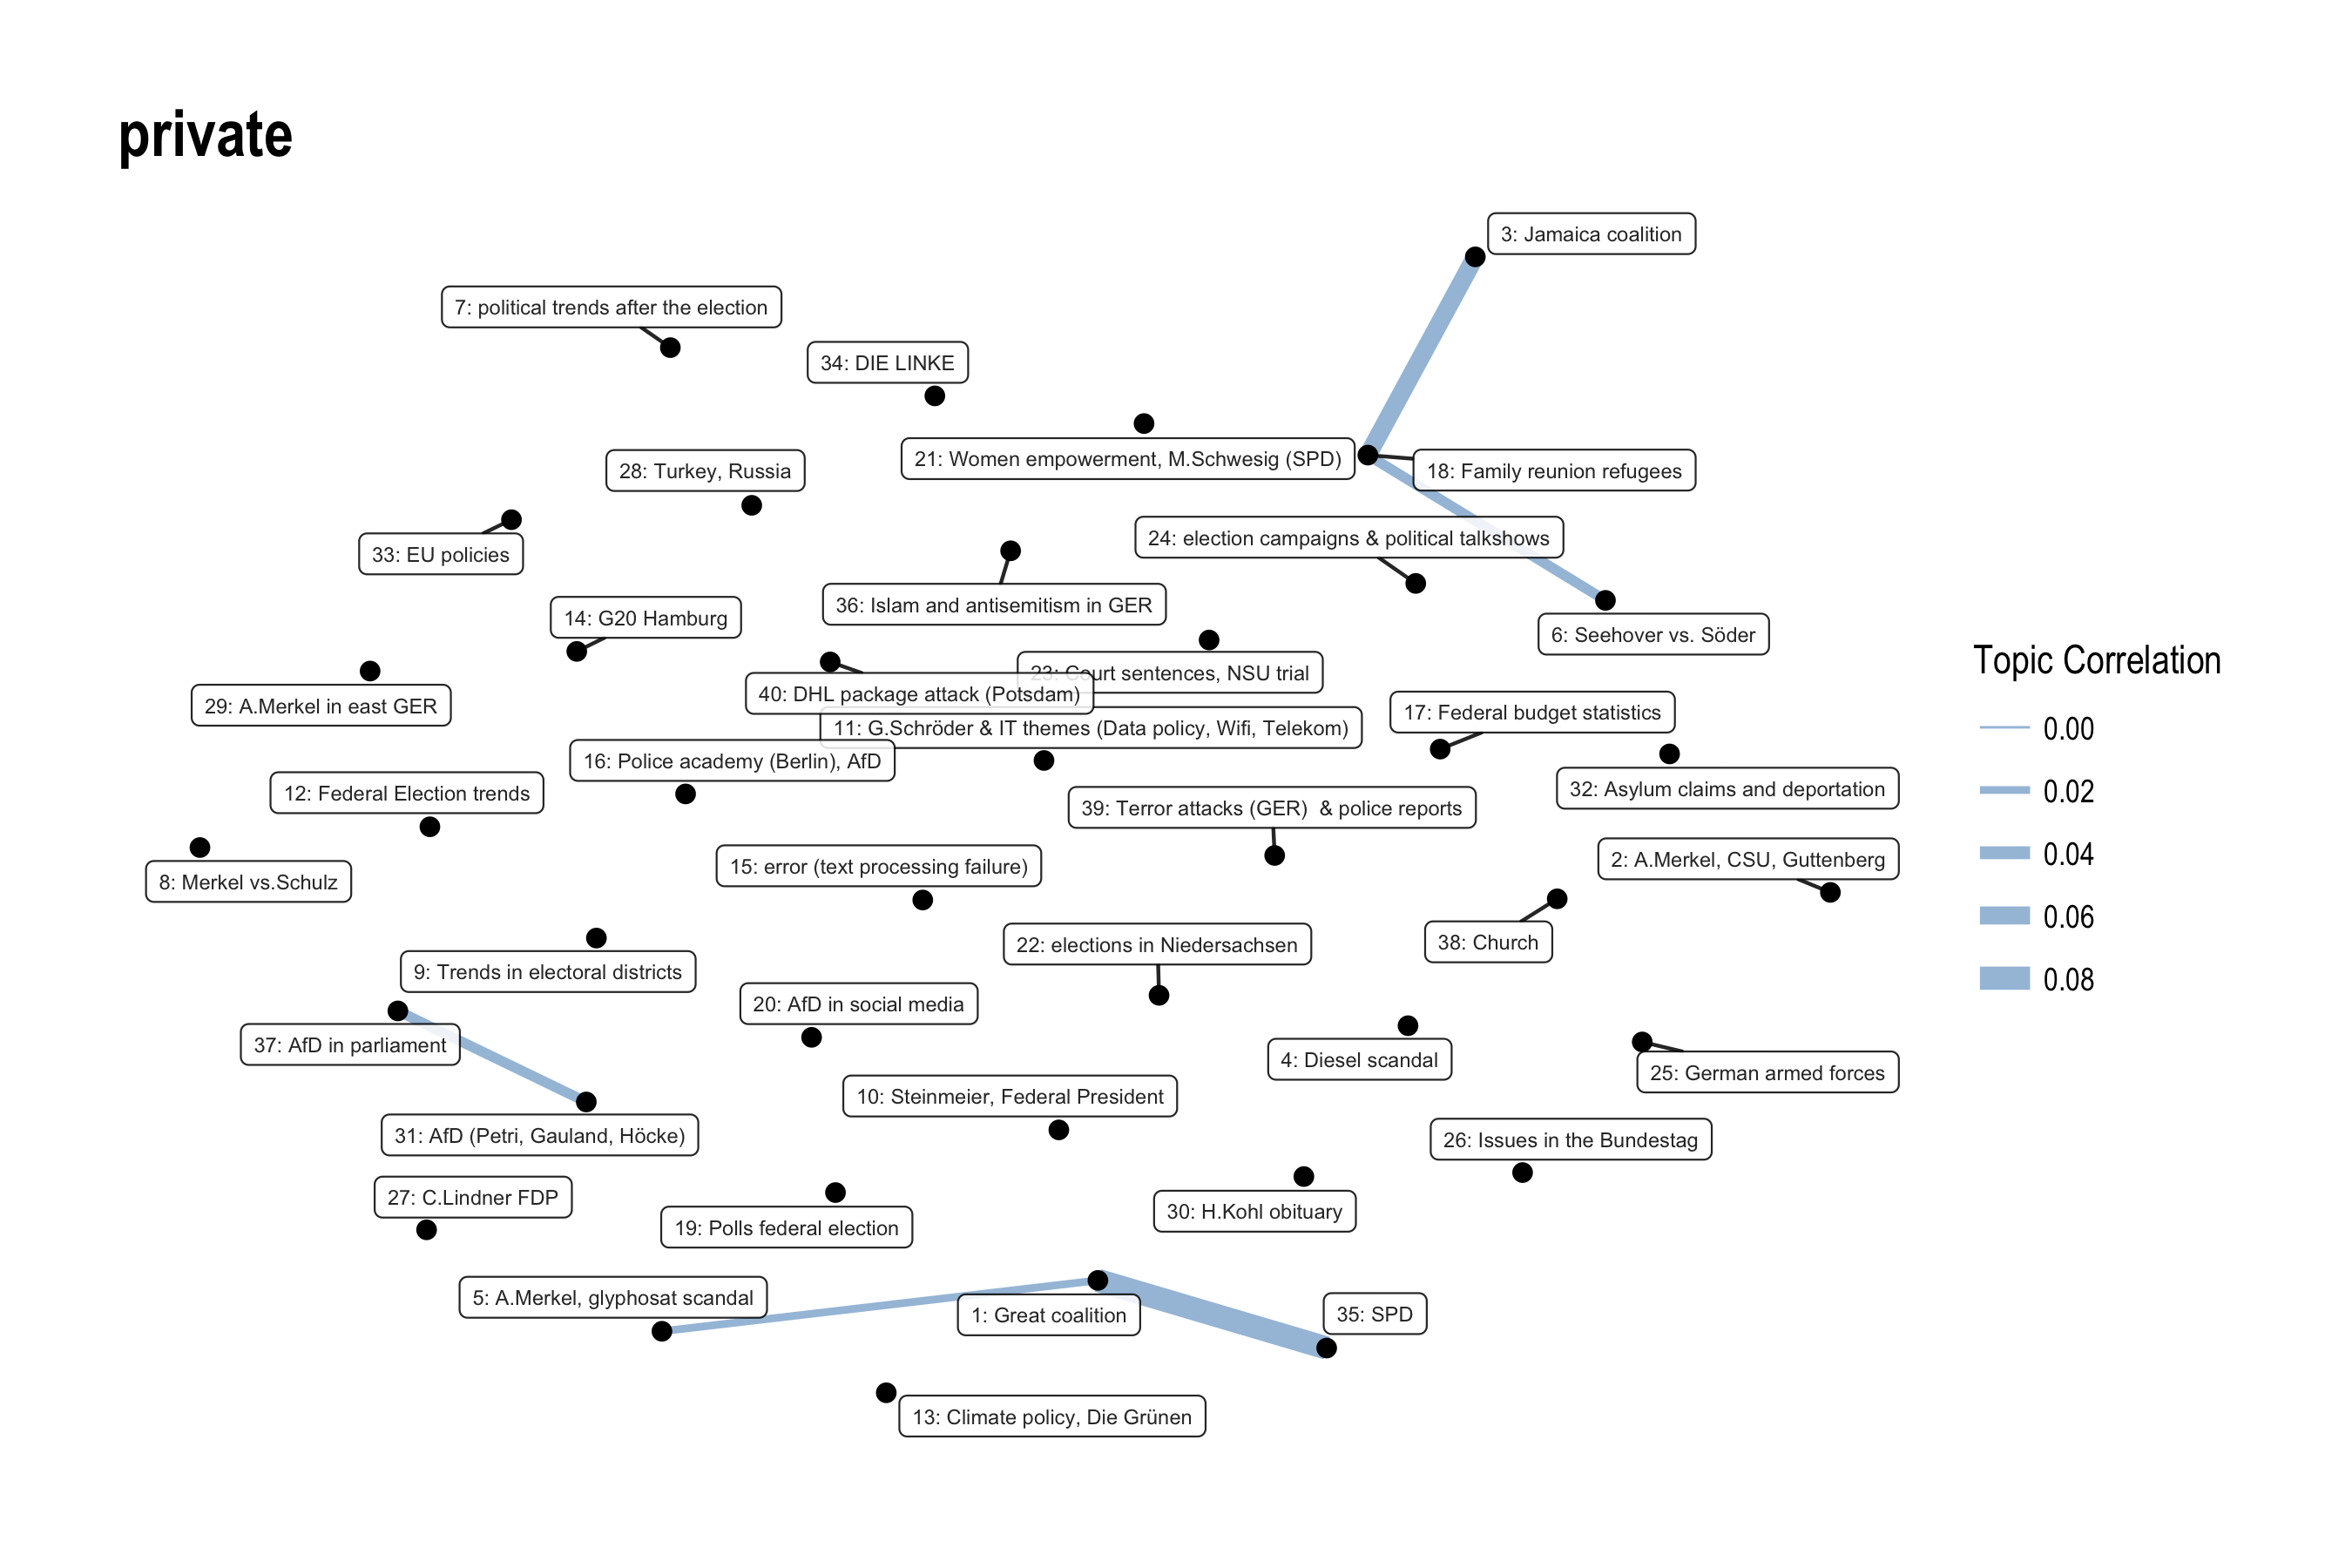
\includegraphics[width=\textwidth]{../figs/corrplot1.png}	
			\subcaption{Private news provider}
		\end{subfigure}
		\begin{subfigure}{.7\textwidth}
			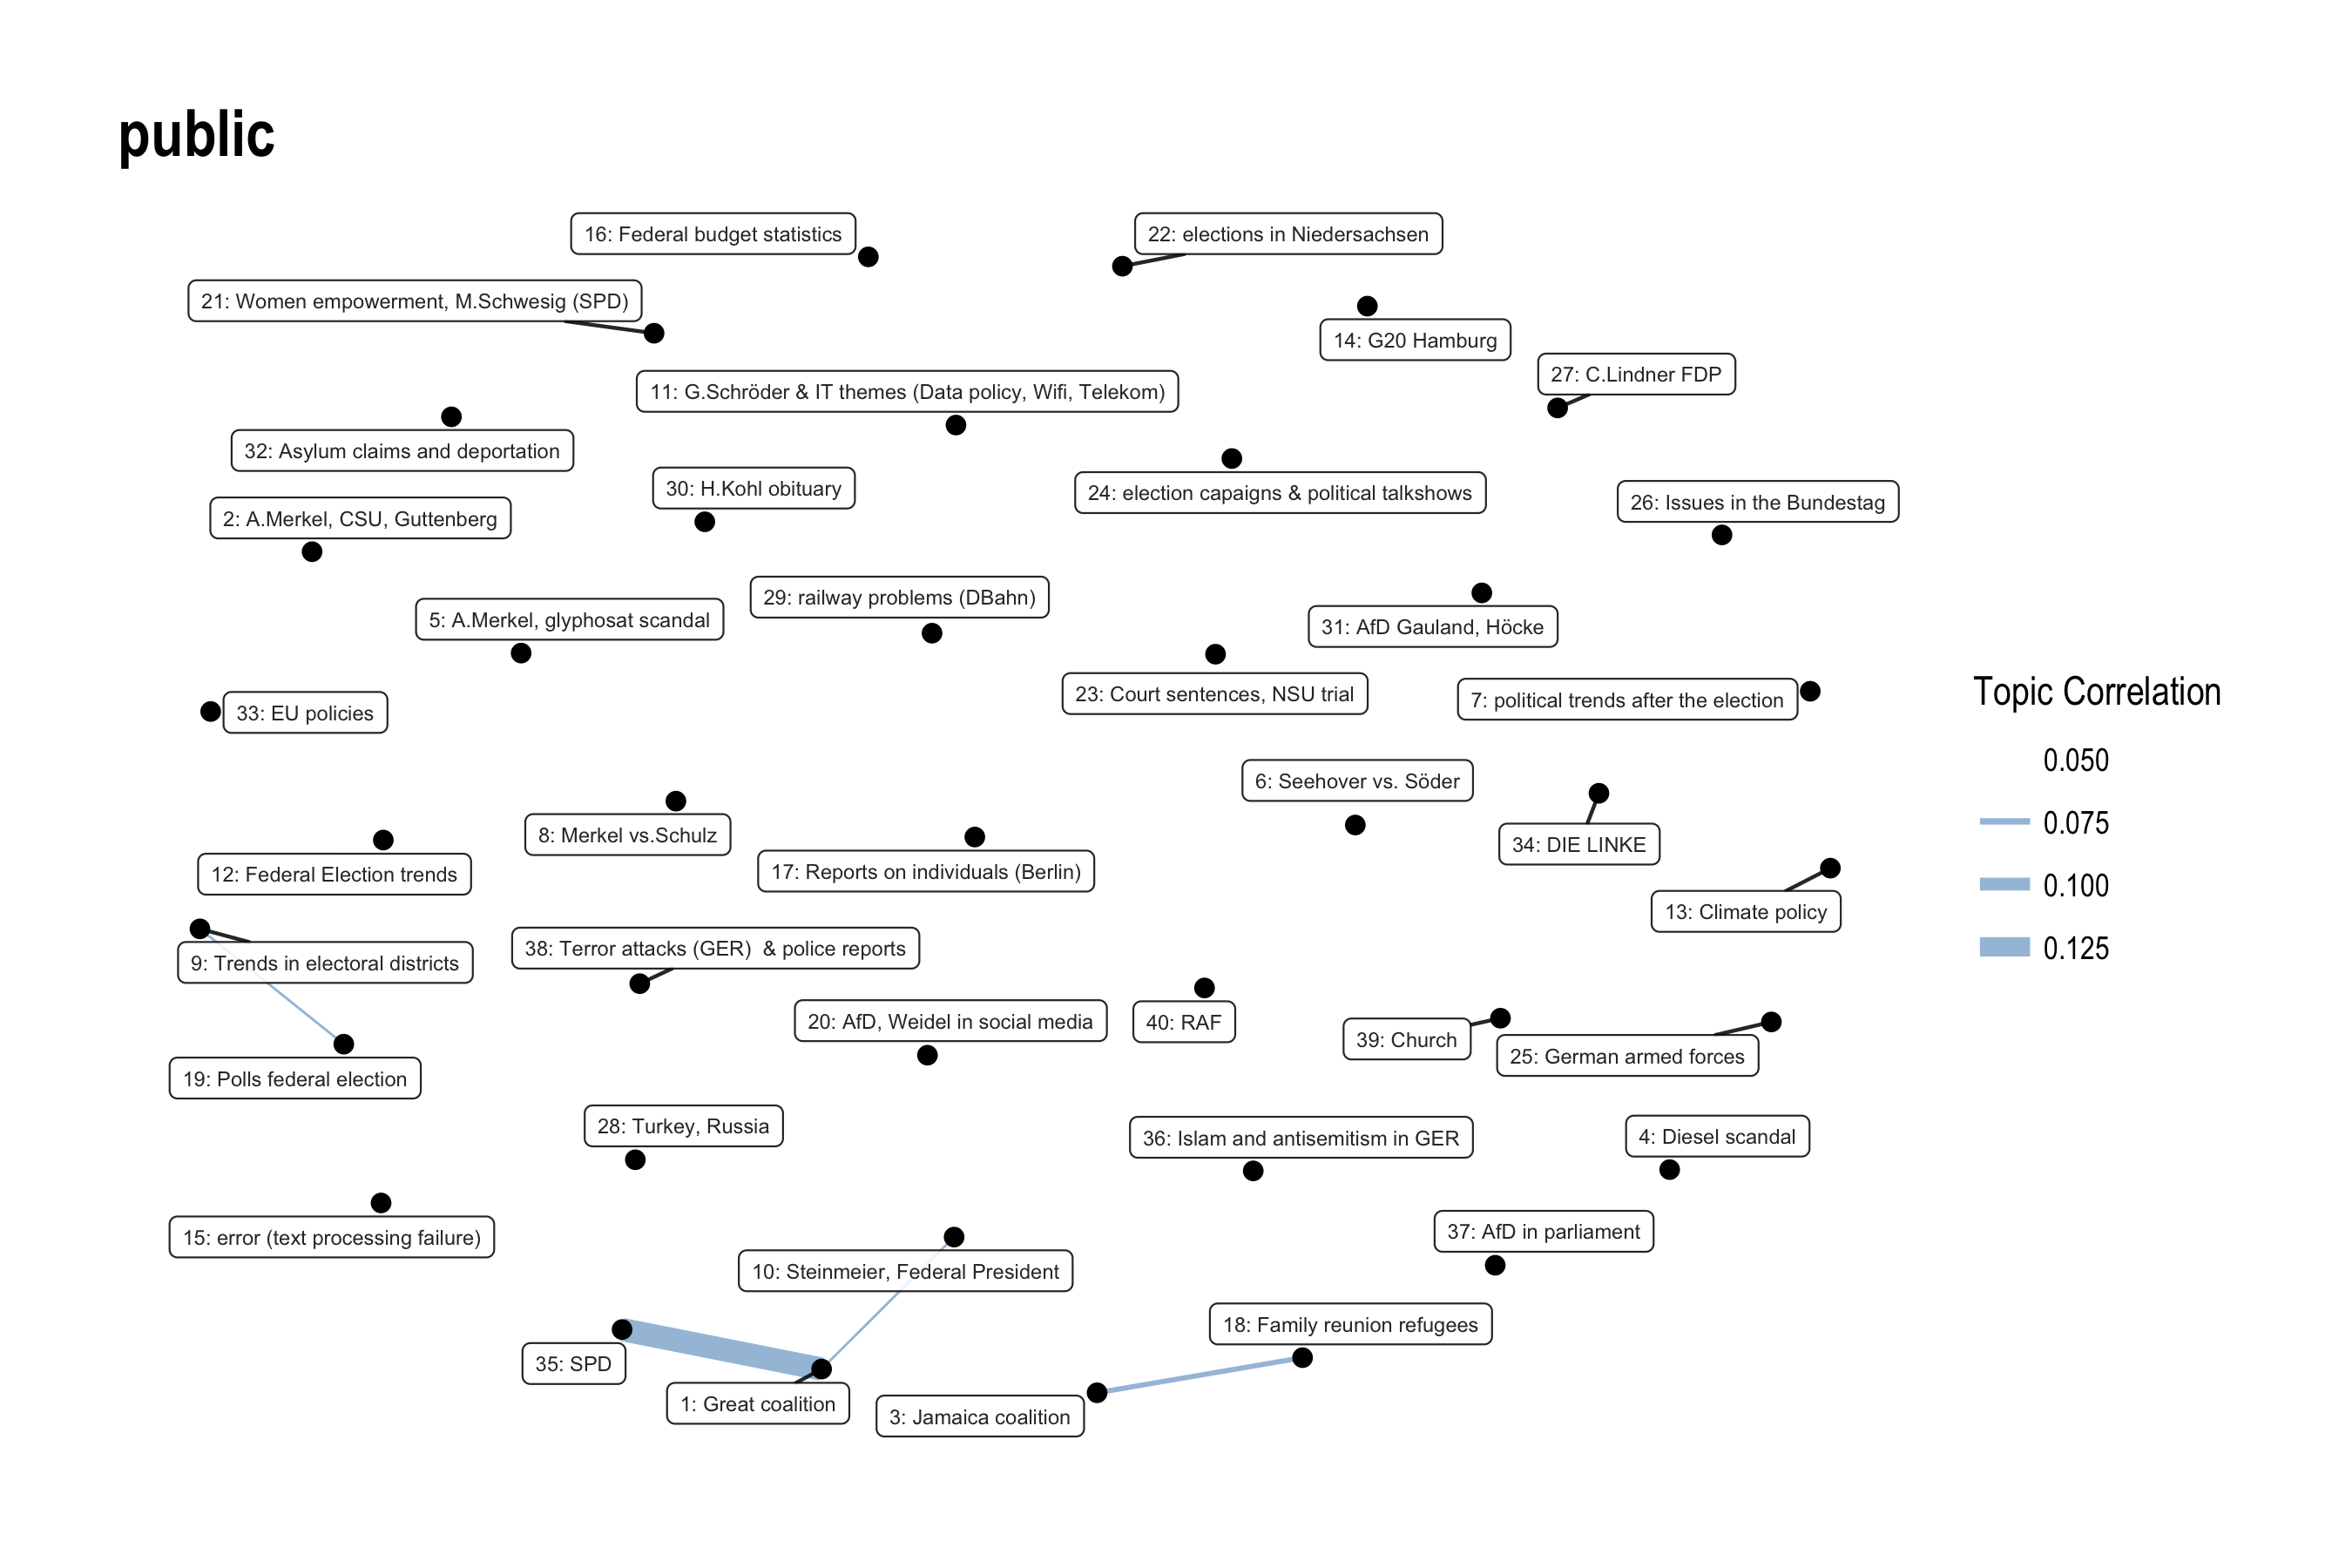
\includegraphics[width=\textwidth]{../figs/corrplot2}
			\caption{Public news provider}	
		\end{subfigure}
		\end{center}
	\label{fig_topic_correlations}
\end{figure}

\textcolor{red}{AUSWERTUNG}

\subsection{Differences in word-topic distributions}\label{subsection_similarity}

Previous topic modeling research try to measure the similarity between topics, comparing the word-topic-distribution between the topics (most of the research uses LDA without metadata, so the word-topic-distribution is the same within the whole corpus). cosine similarity \citep{he_detecting_2009}, \citep{ramage_labeled_2009}, Kullback-Leibler (KL) \citep{newman_distributed_2009}, \citep{wang_mining_2009} and the average Log Odds Ratio \citep{chaney_visualizing_2012} are frequently used metrics to compare word probability distributions. \citet{kim_topic_2011} compare six popular similarity metrics in terms of log likelihood of data, concluding that Jensen-Shannon Divergence (the symmetric variation of KL divergence) is best in terms of performance and generality. 

Since a topic is a multinomial distribution over the vocabulary, where $\beta_{kvi}$ indicates the probability of observing word $v$ in topic $k$ for covariate level $i$, we can analyze how similar a topic $k$ is for different levels of covariates. More precisely, we can calculate the similarity between $\beta_{kvi}$ and $\beta_{kvj}$. I use each row of that matrix (corresponding to each topic) to calculate the similarity of the word-topic distribution between the public and private media using the square root of the Jensen-Shannon (JS) Divergence. I will compare this metric with a set of other similarity measures recently used in the literature to measure the difference between word-topic distributions: The Kullback-Leibler (KL) divergence (\citet{newman_distributed_2009}, \citet{wang_mining_2009}), the cosine similarity (\citet{he_detecting_2009}, \citet{ramage_labeled_2009}) and the difference of the $L1$ norm of the vectors \citep{roberts_navigating_2016}. Before the results are presented, I will briefly explain these measures before I proceed to the results.

Essentially, the KL divergence is the expectation of the log difference between probabilities $a$ and $b$. It can be defined as:

\begin{align*}
	D_{KL}(a,b)=\sum_{i=1}^T a_i \text{ln} \frac{a_i}{b_i},
\end{align*}

where $D_{kl} \to 0$ indicates stronger similarities. However, since the KL divergence is not symmetric, it cannot be used to measure the distance between two distributions, but as a divergence measure.

The Jensen-Shannon Divergence is a positive definite measure, satisfying the following conditions: $D_{js}(a,b) \geq 0$, $D_{js}(a,b)=0$ iff $(a=b)$. It is also symmetric: $D_{js}(a,b)=D_{js}(b,a)$. The Jensen-Shannon distance $D_{js}(a,b)$ between the two distributions is defined as:

\begin{align*}
	D_{js}(a,b)=\frac{1}{2}D_{KL}(a,\frac{a+b}{2})+\frac{1}{2}D_{KL}(b,\frac{a+b}{2})
\end{align*}

where $D_{KL}$ is the Kullback-Leibler divergence. Since $D_{js}$ does not satisfy the triangular inequality condition $D_{js}(a,c)\leq D_{js}(a,c)+D_{js}(b,c)$, the JSD is not considered to be a real distance metric. However, we can use the square root of JSD as a real distance metric \citep{endres_new_2003}.

\citet{roberts_navigating_2016} use the $L_1$ norm of the word-topic distributions to compare topics from different models. The $L_1$ norm is the sum of the absolute value of the difference between two vectors. Its defined as

\begin{align*}
	L_1=\sum_{i=1} |a_i-b_i|
\end{align*}

this measure has a range of $[0,2]$, where $ L_1 \to 0$ indicates strong similarities. \citet{roberts_navigating_2016} compare this measure with a cosine similarity metric, which is essentially the dot product rescaled by the $L_2$ norm of the vectors and is defined as.

\begin{align*}
	\text{cos}(\theta)=\frac{\sum_{i=1}a_i b_i}{\sqrt{\sum_{i=1}a_i^2}\sum_{i=1}b_i^2}
\end{align*}

However, different to the above mentioned metrics the cosine similarity has a range of $[0,1]$ and $cos(\theta) \to 0$ indicate less similarity.

Figure \ref{fig_distance} displays the different distance measures 

\begin{figure}[H]
	\begin{center}
		\caption{Similarity measures of word-topic probabilities}
		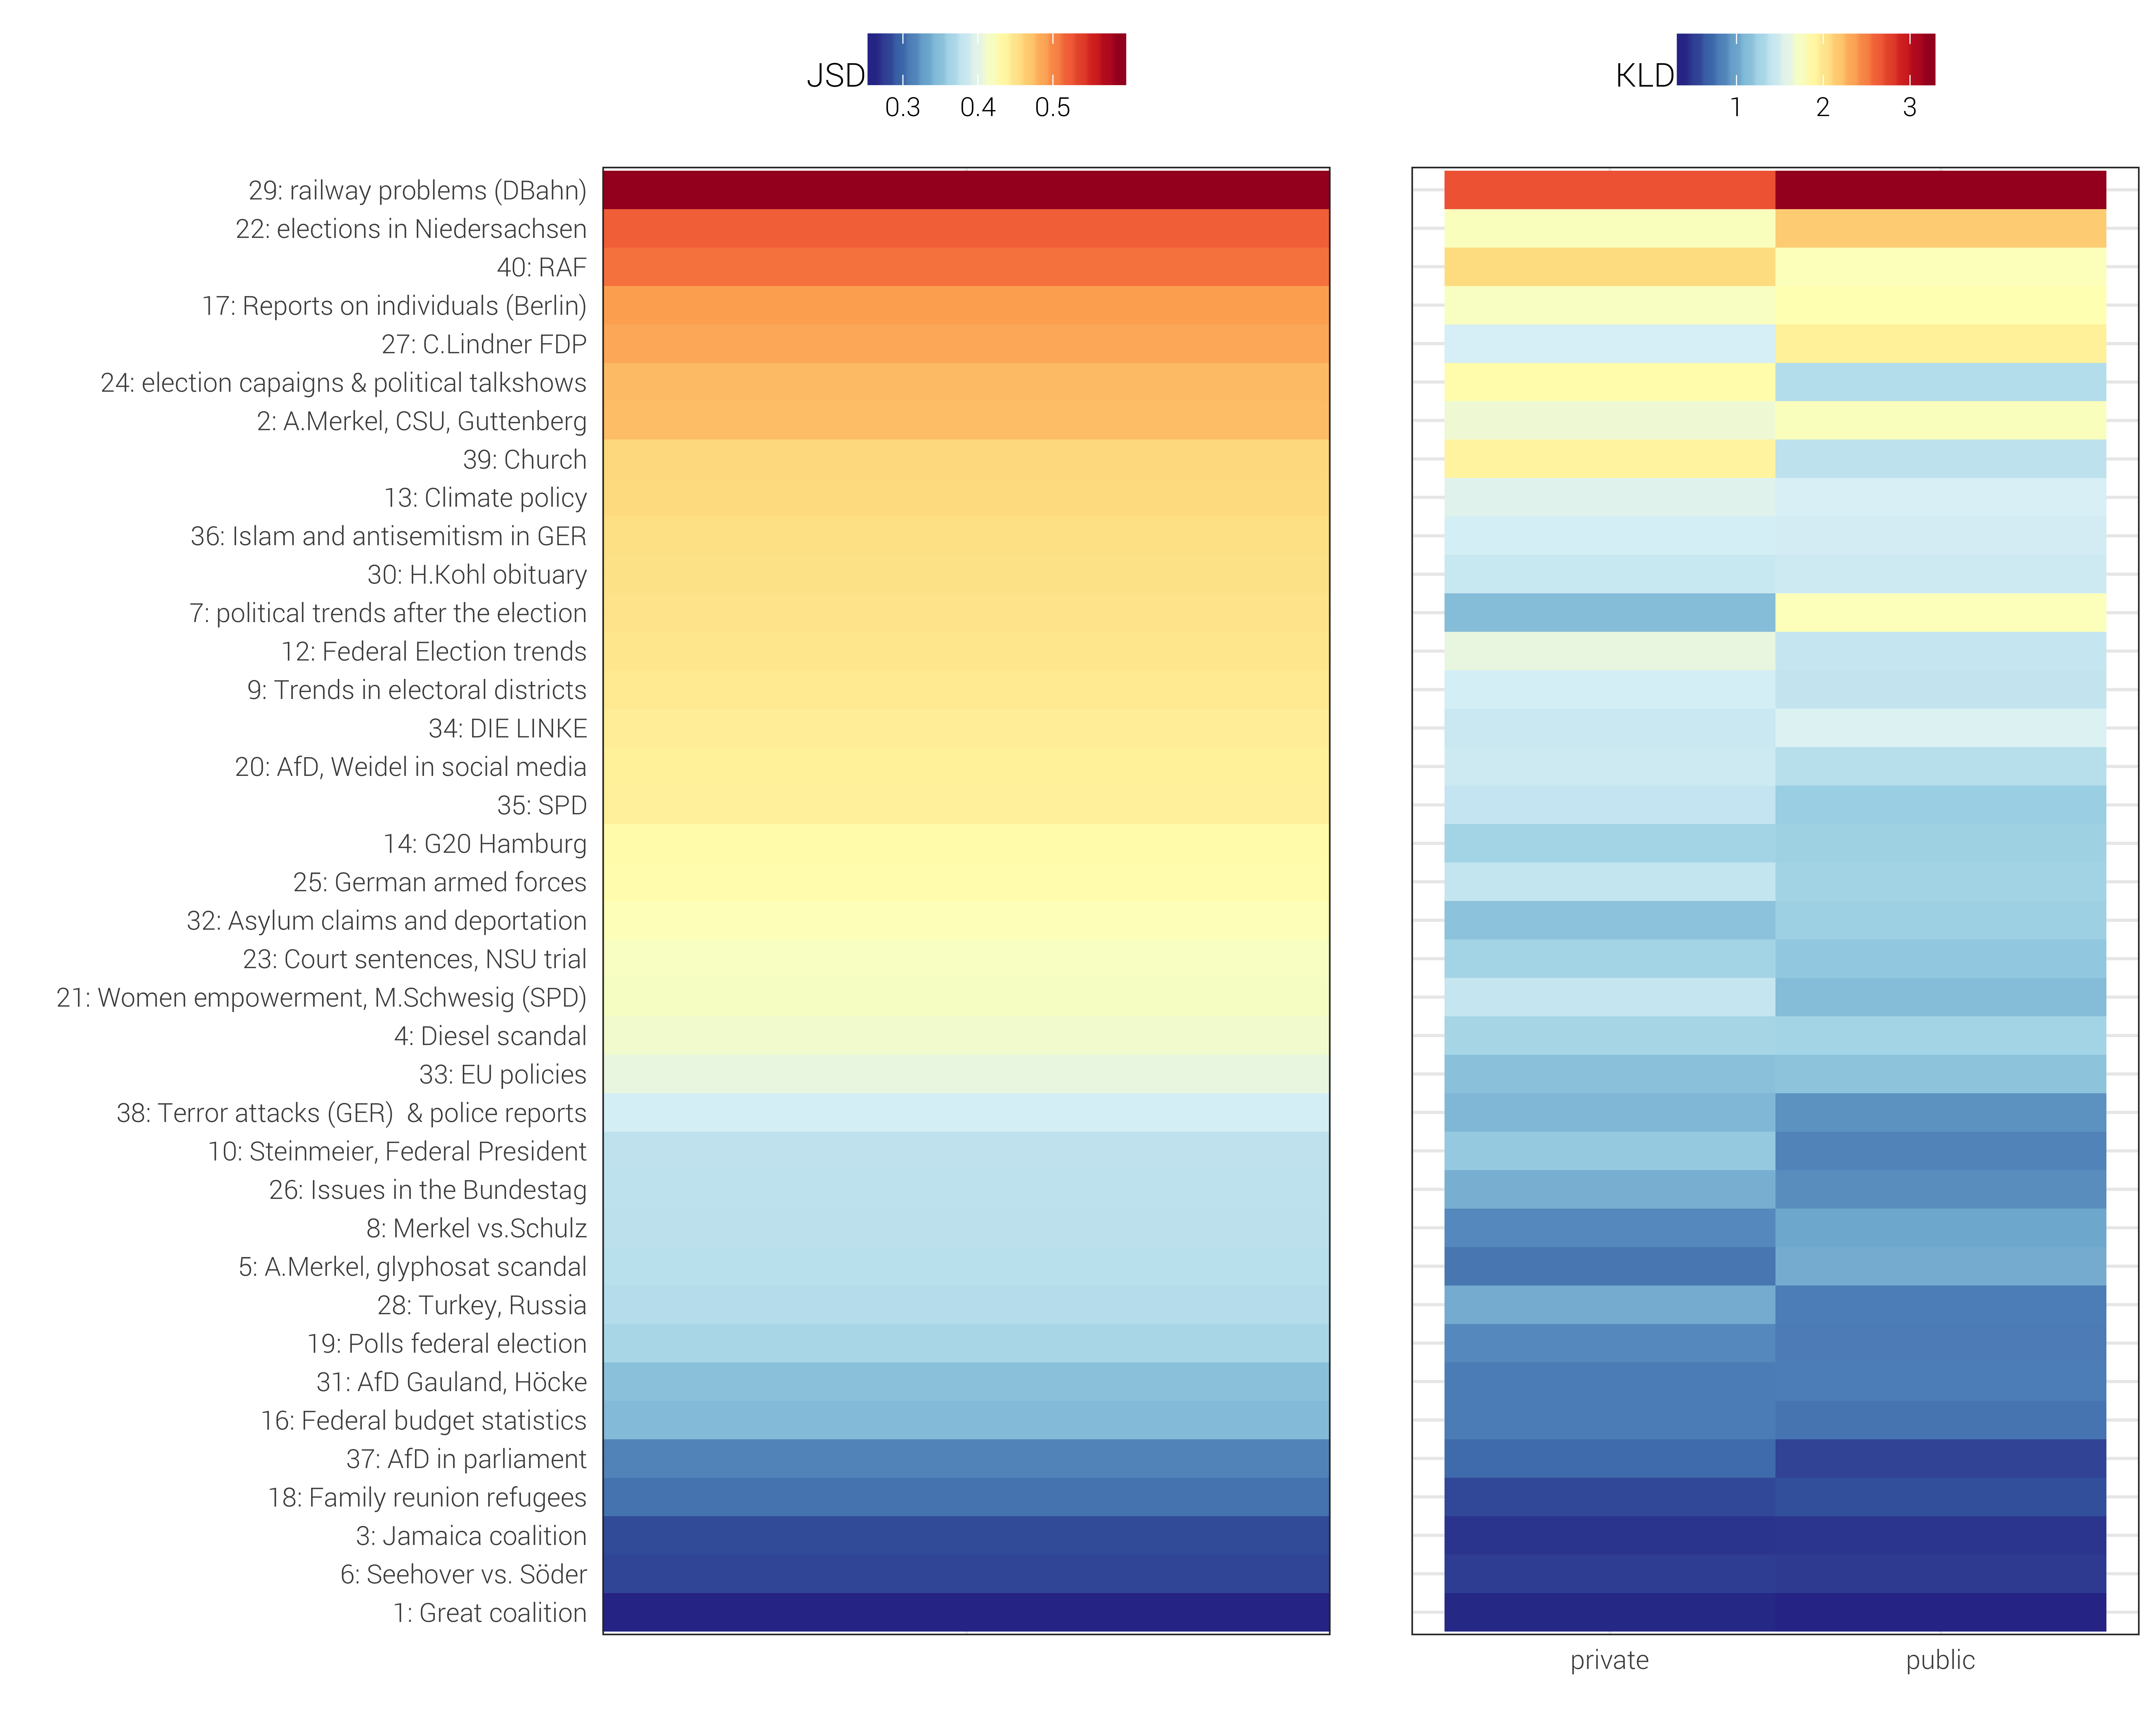
\includegraphics[width=\textwidth,keepaspectratio]{../figs/distance}
		\label{fig_distance}
	\end{center}
\end{figure}


% ----------------------
% Regression
% ----------------------
\section{Causal relationship between topics and social media shares.}\label{ch_regression}

%\begin{figure}[H]
%\centering
%	\caption{Sum of Facebook shares by topic}
%	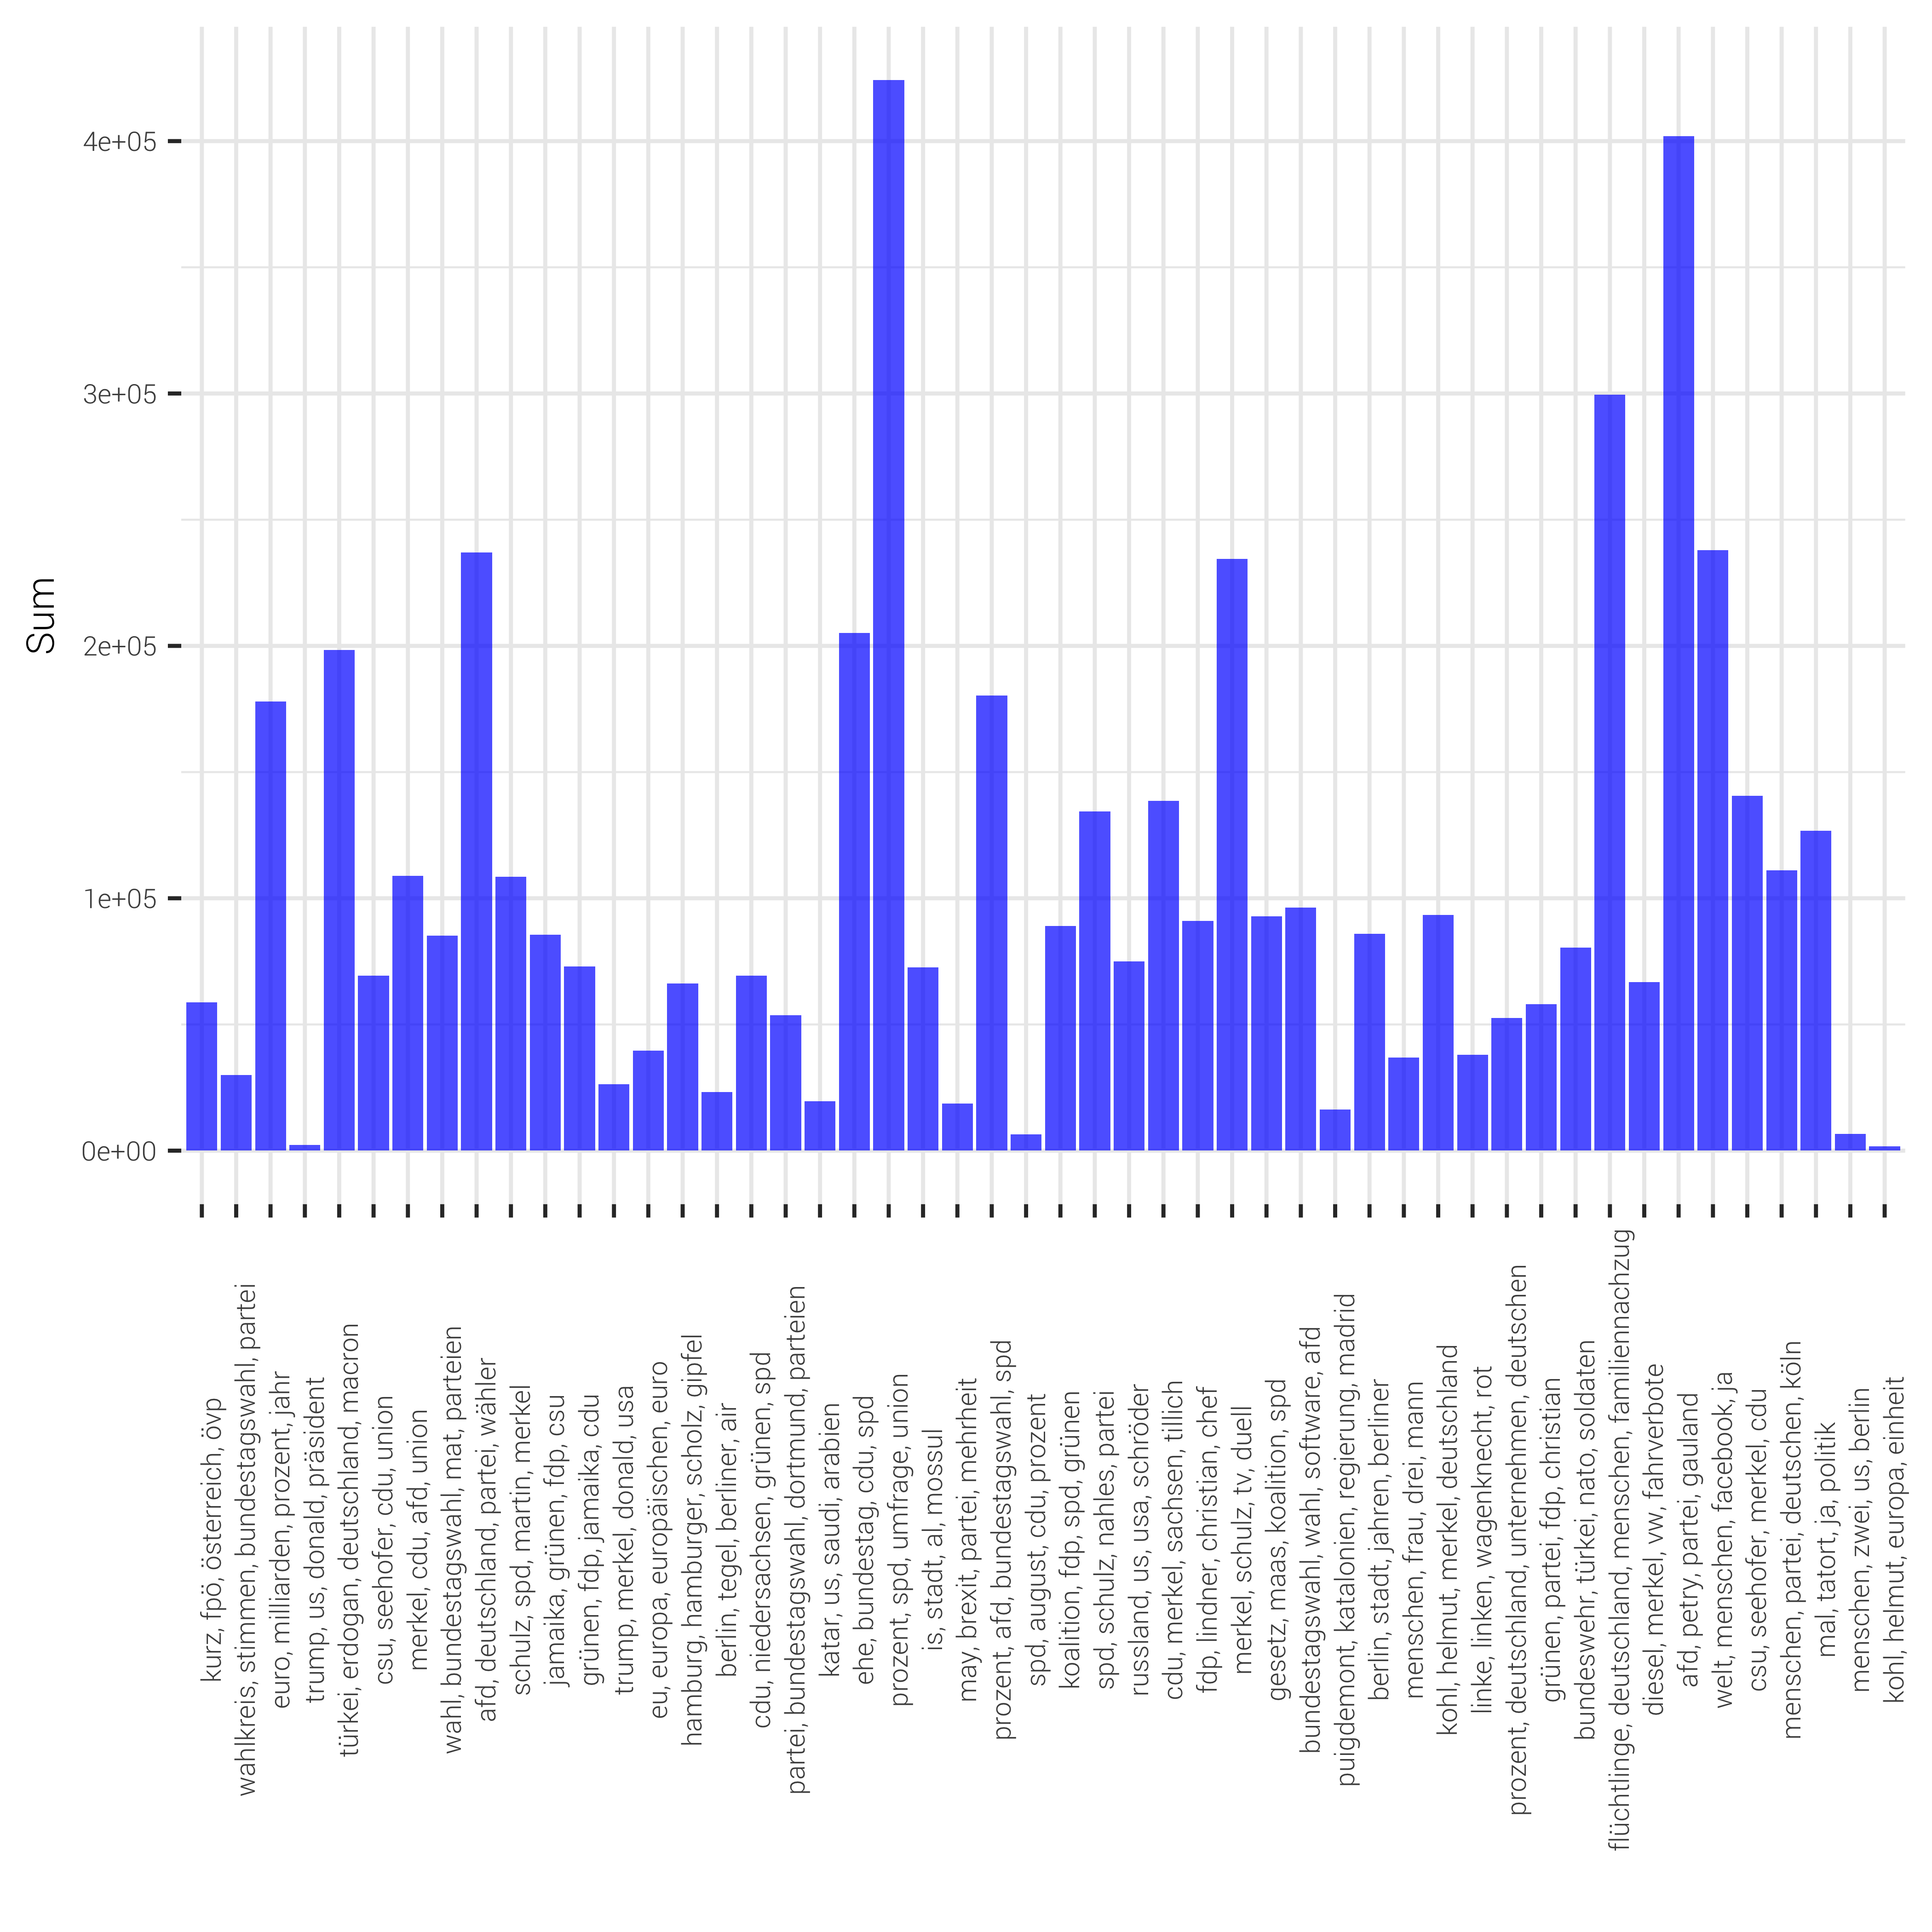
\includegraphics[width=\textwidth]{../figs/fb_shares_topics.png}	
%	\label{fig_fb_shares_topic}
%\end{figure}

In order to answer the primary question of this paper, which topics are more often shared in social networks, we assign a single topic to each article. The examination of the topic probability distribution revealed that most documents are assigned a unique topic with a probability of 50\% and higher (see figure \ref{fig_gamma}), so that we can classify each document based on which topic has the highest probability. We keep only those documents, where the posterior probability of this topic is greater or equal than 0.5 which left us with 6565 documents. Figure \ref{fig_topic_timeline} shows the amount of articles to which a certain topic has been assigned over time. Some of the topics exhibit distinct peaks in the timeline. Topics 11 and 14 deal with the elections, although topic 11 tends to be more about incidents related to the AfD. This graph also illustrates the difference between topic 6 and 17, which have similar labels: topic 6 classifies articles before the negotiations for a "Jamaika" coalition failed, while topic 17 describes the articles written after failure. The highest peak can be found for topic 9, which classifies articles to the riots during the G20 summit. It becomes apparent that more articles deal with riots than with the political content of the summit (topic 8). 

The proportion of zeros in the independent variable (number of Facebook shares) is about 15\%. Figure \ref{fig_fb_shares} reveals that within the bin of 0-1 facebook shares, nearly all articles are published by stern.de. 

\begin{figure}[H]
	\caption{}
	\begin{center}
		\begin{subfigure}[normla]{0.49\textwidth}
			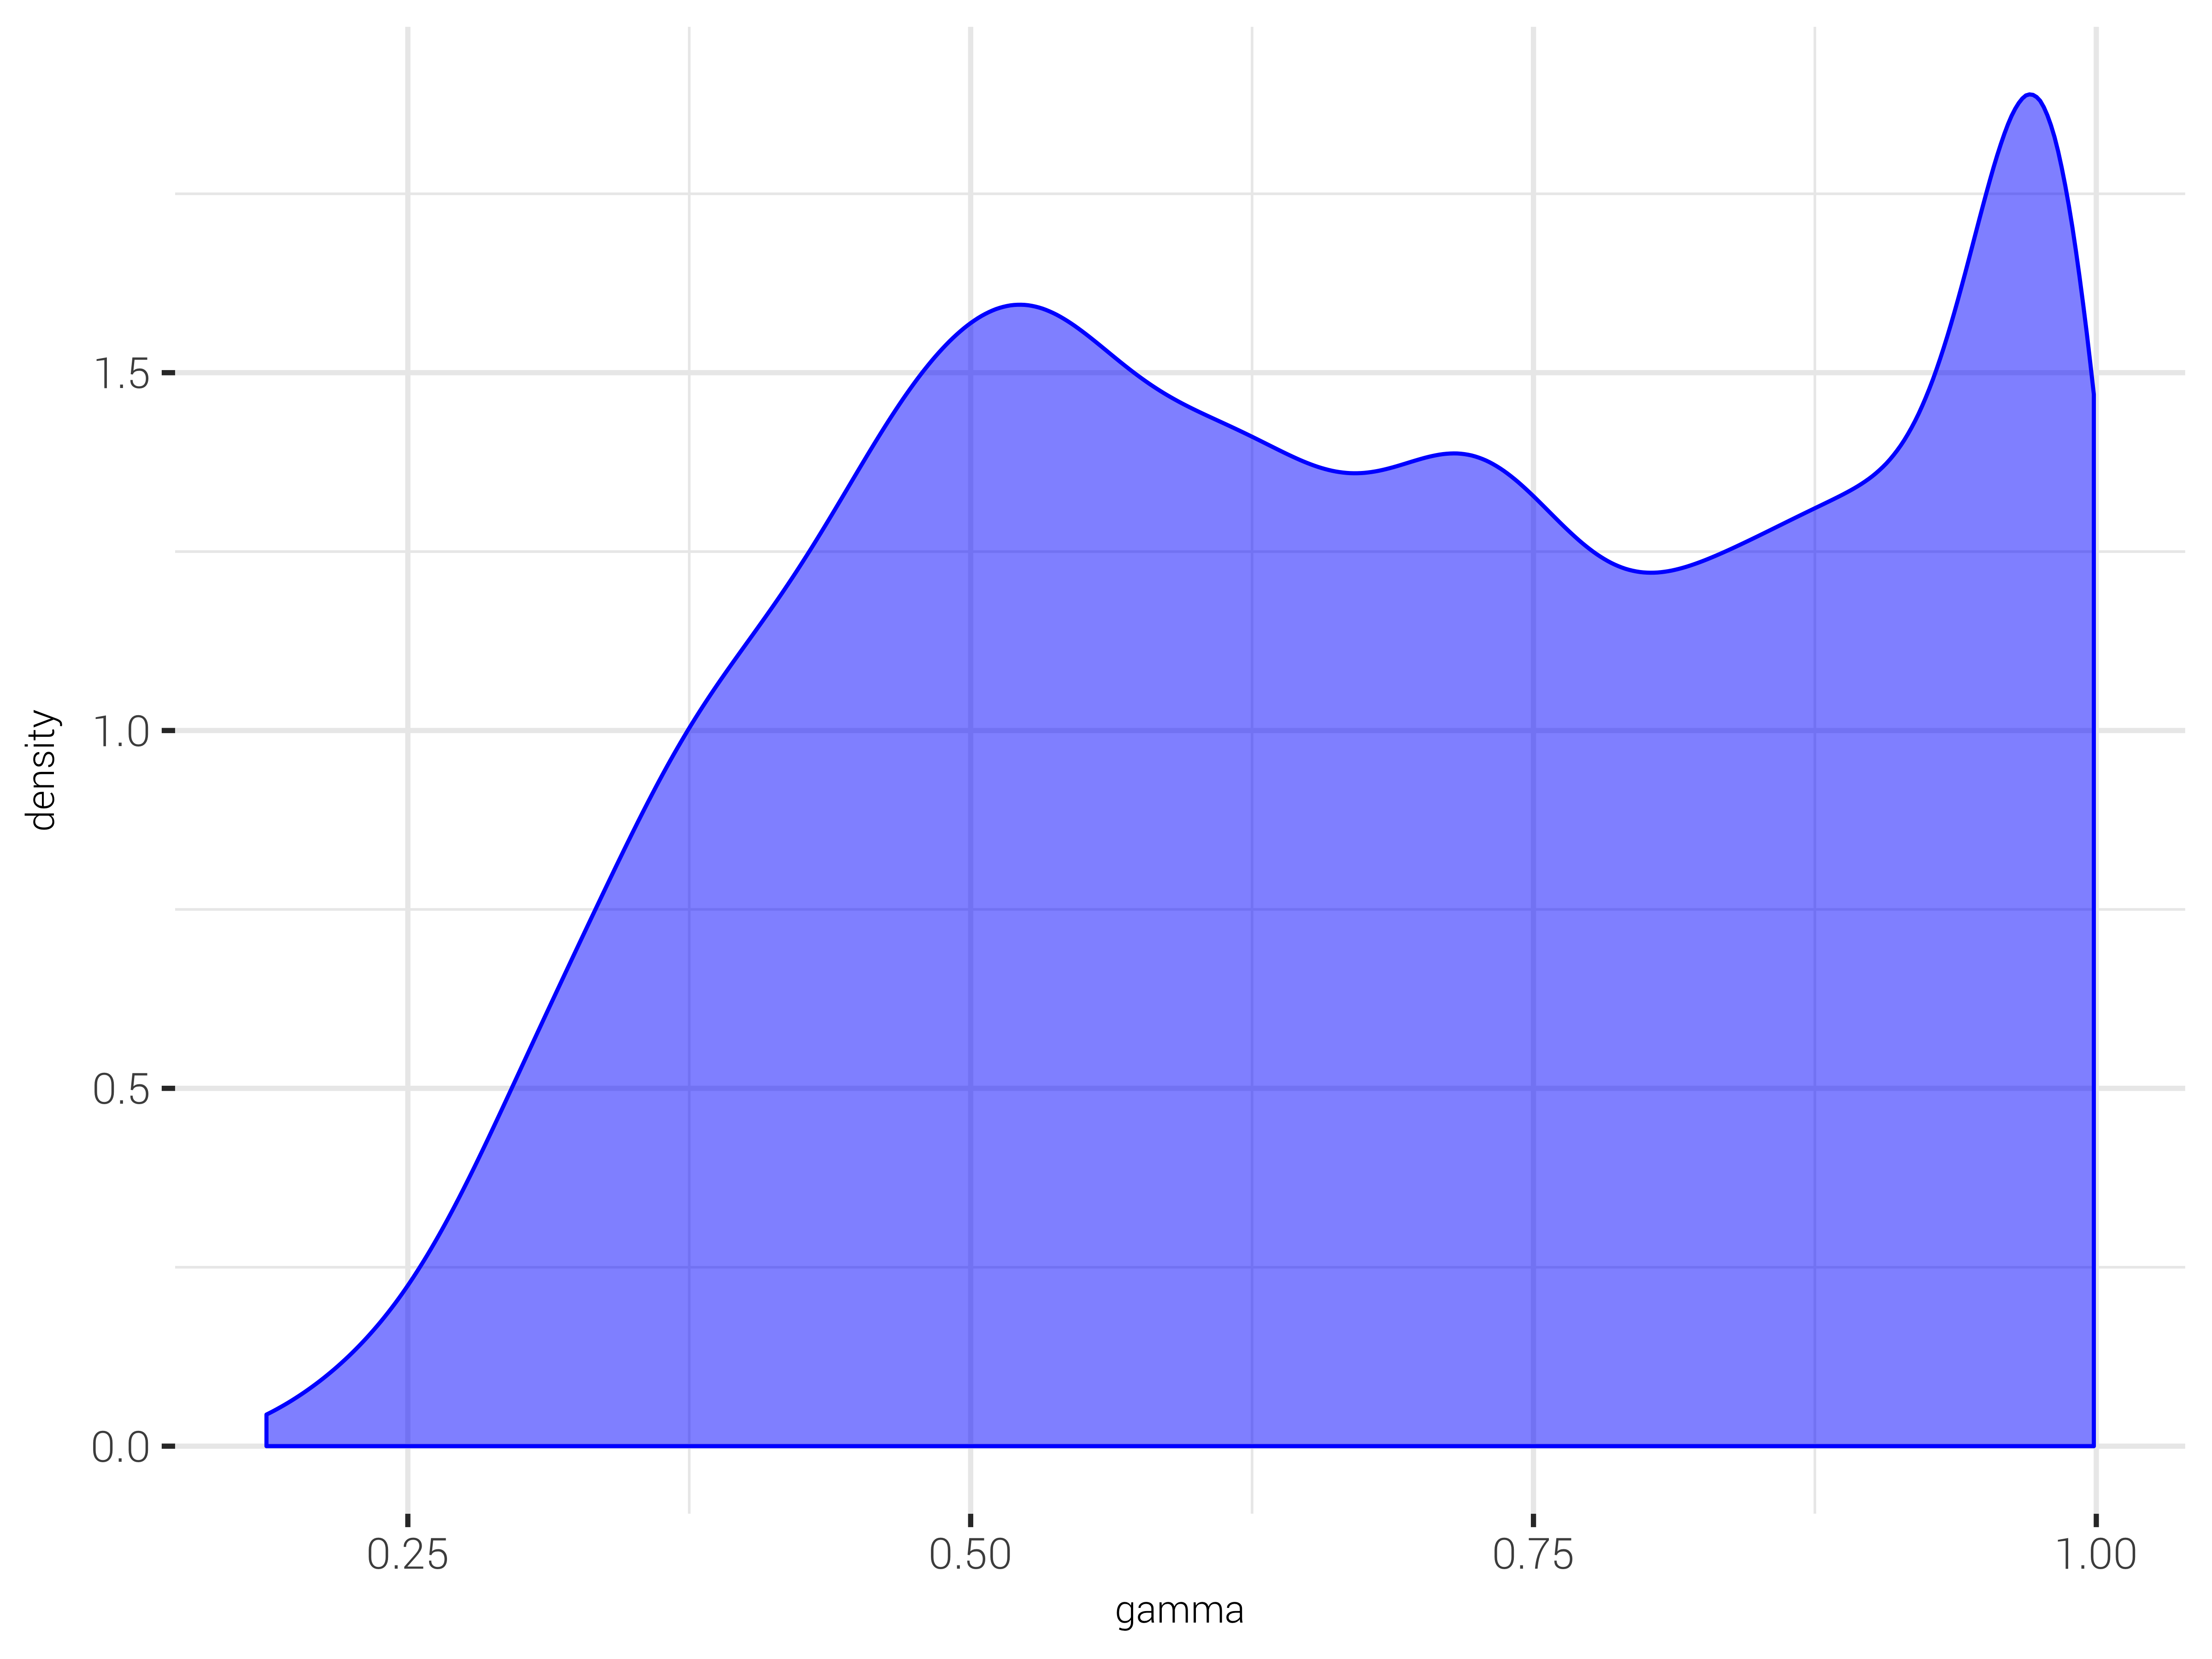
\includegraphics[width=\textwidth,keepaspectratio]{../figs/gamma_dist.png}
			\caption{Density of Top-Topics posterior probability}
			\label{fig_gamma}
		\end{subfigure}
		\begin{subfigure}[normla]{0.49\textwidth}
			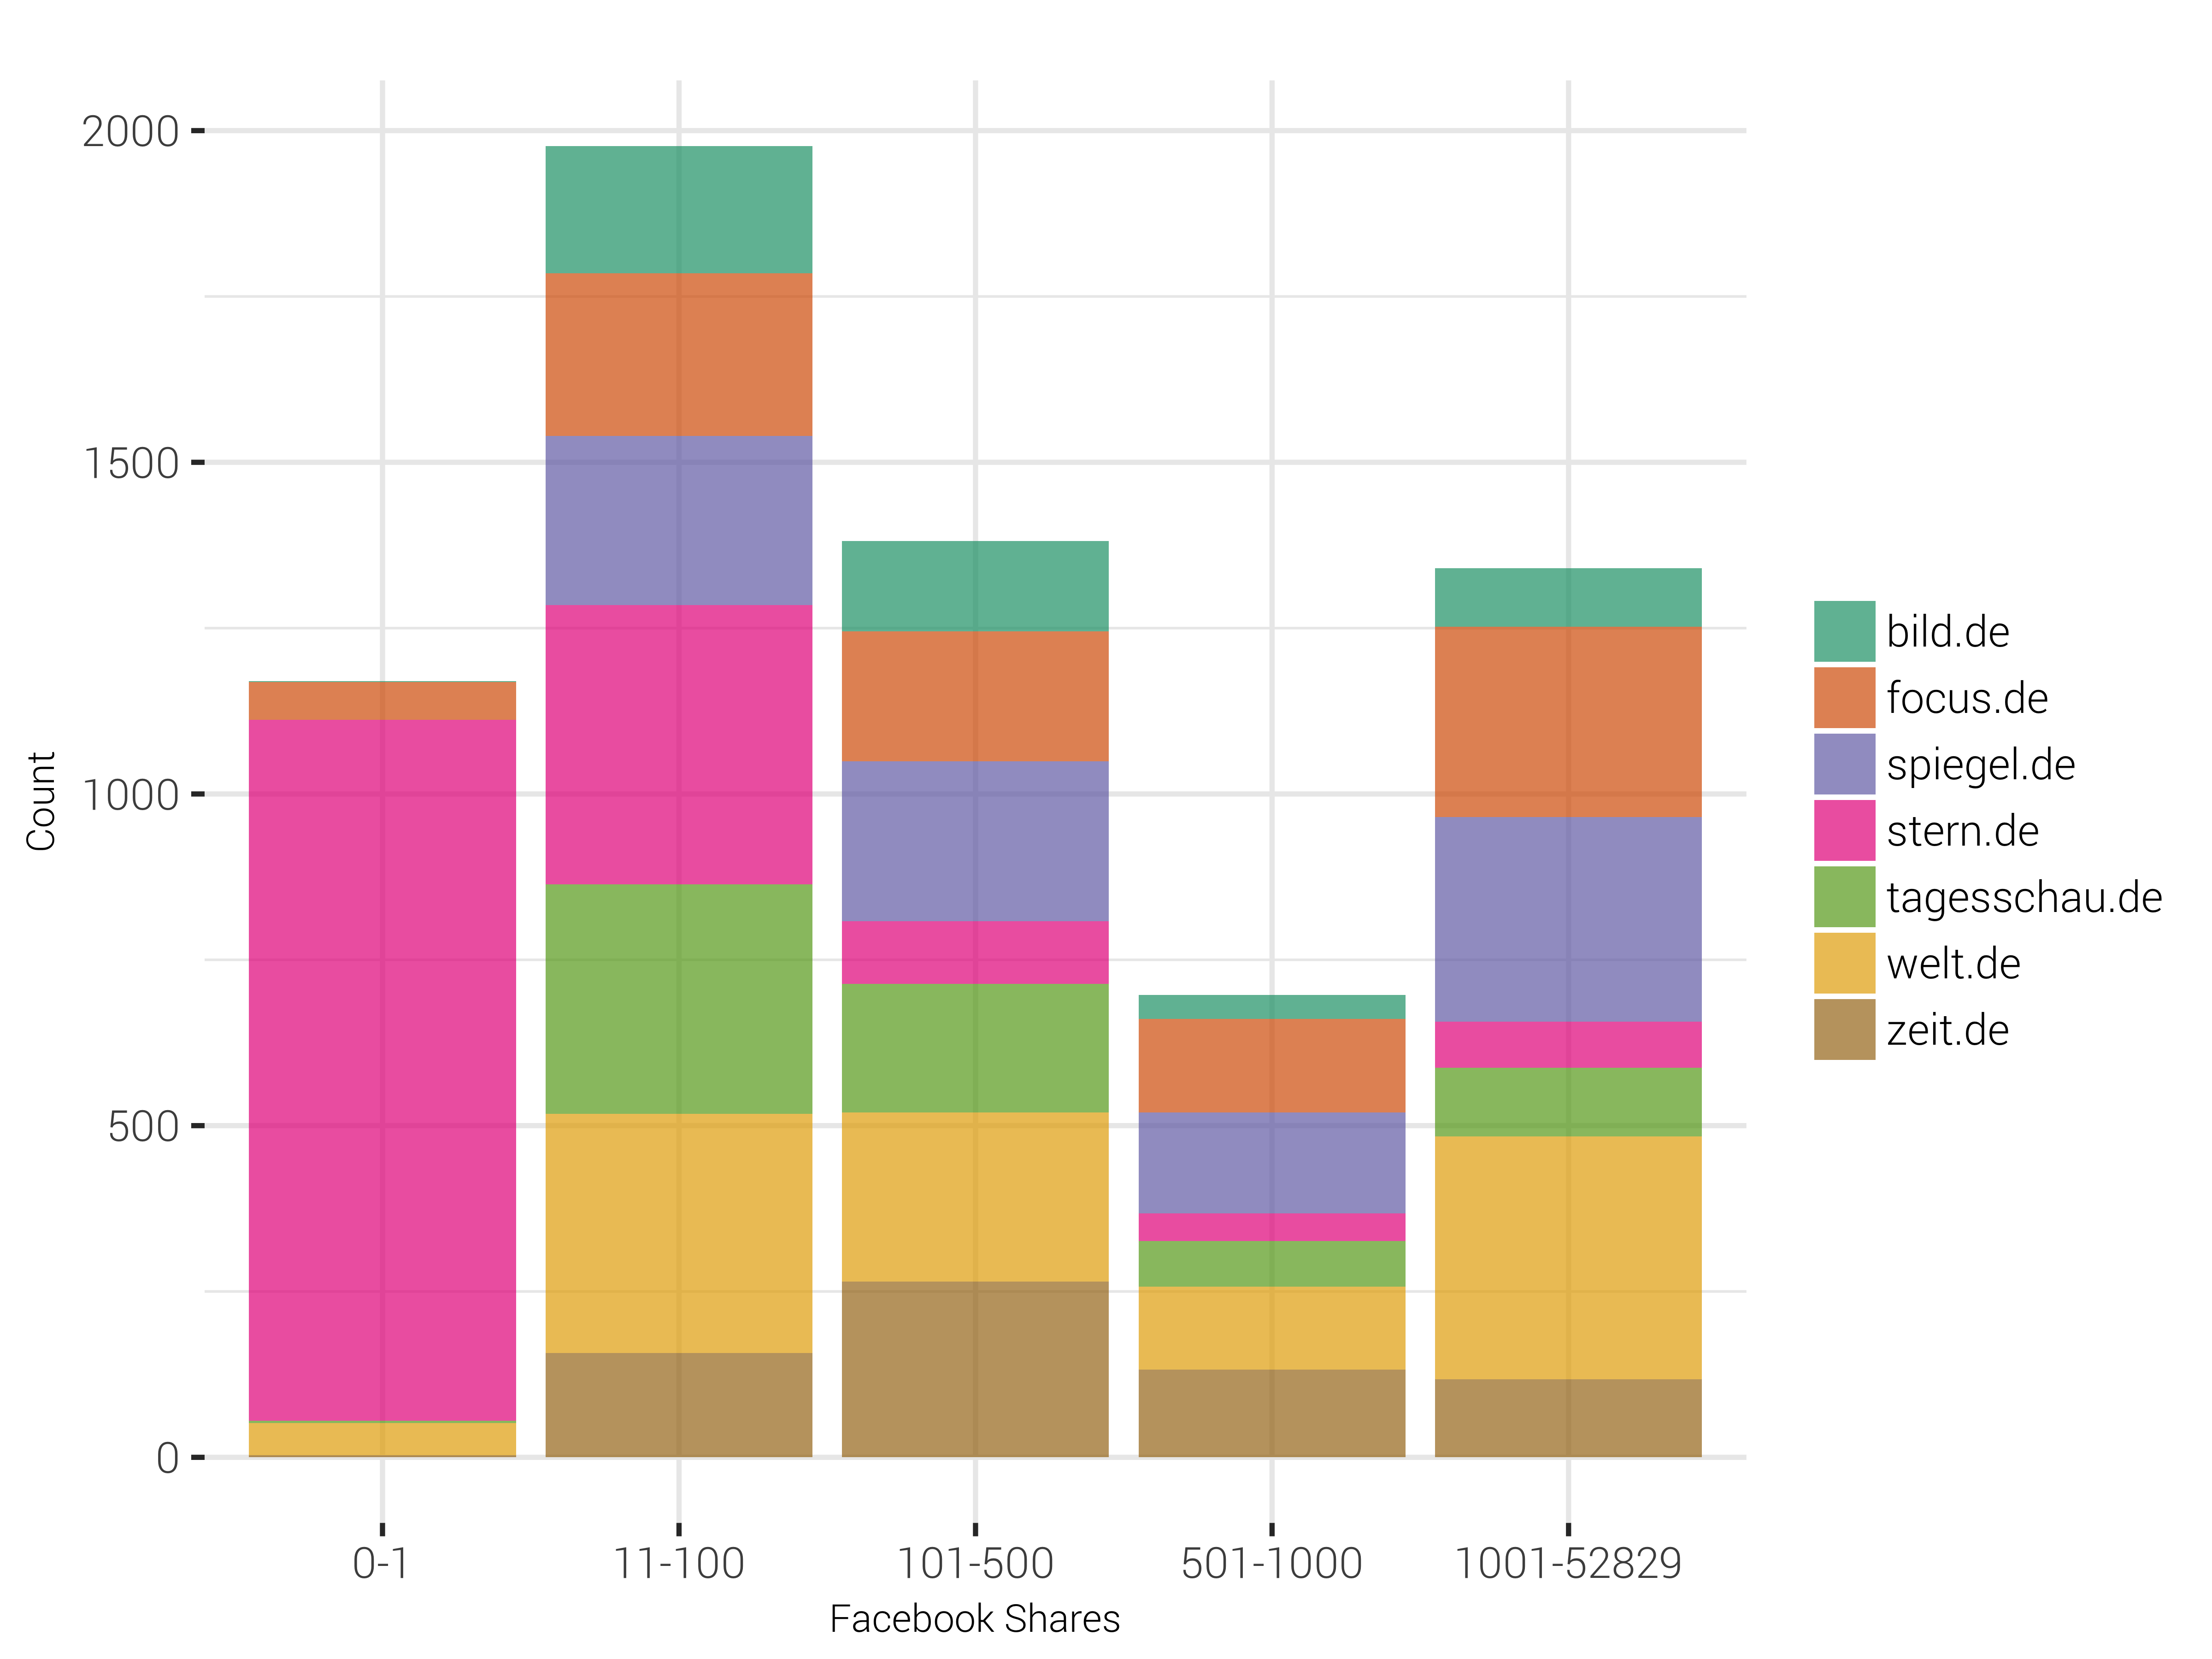
\includegraphics[width=\textwidth,keepaspectratio]{../figs/facebook_shares.png}
			\caption{Grouped Facebook Shares}
			\label{fig_fb_shares}
		\end{subfigure}
		\begin{subfigure}[normla]{0.9\textwidth}
			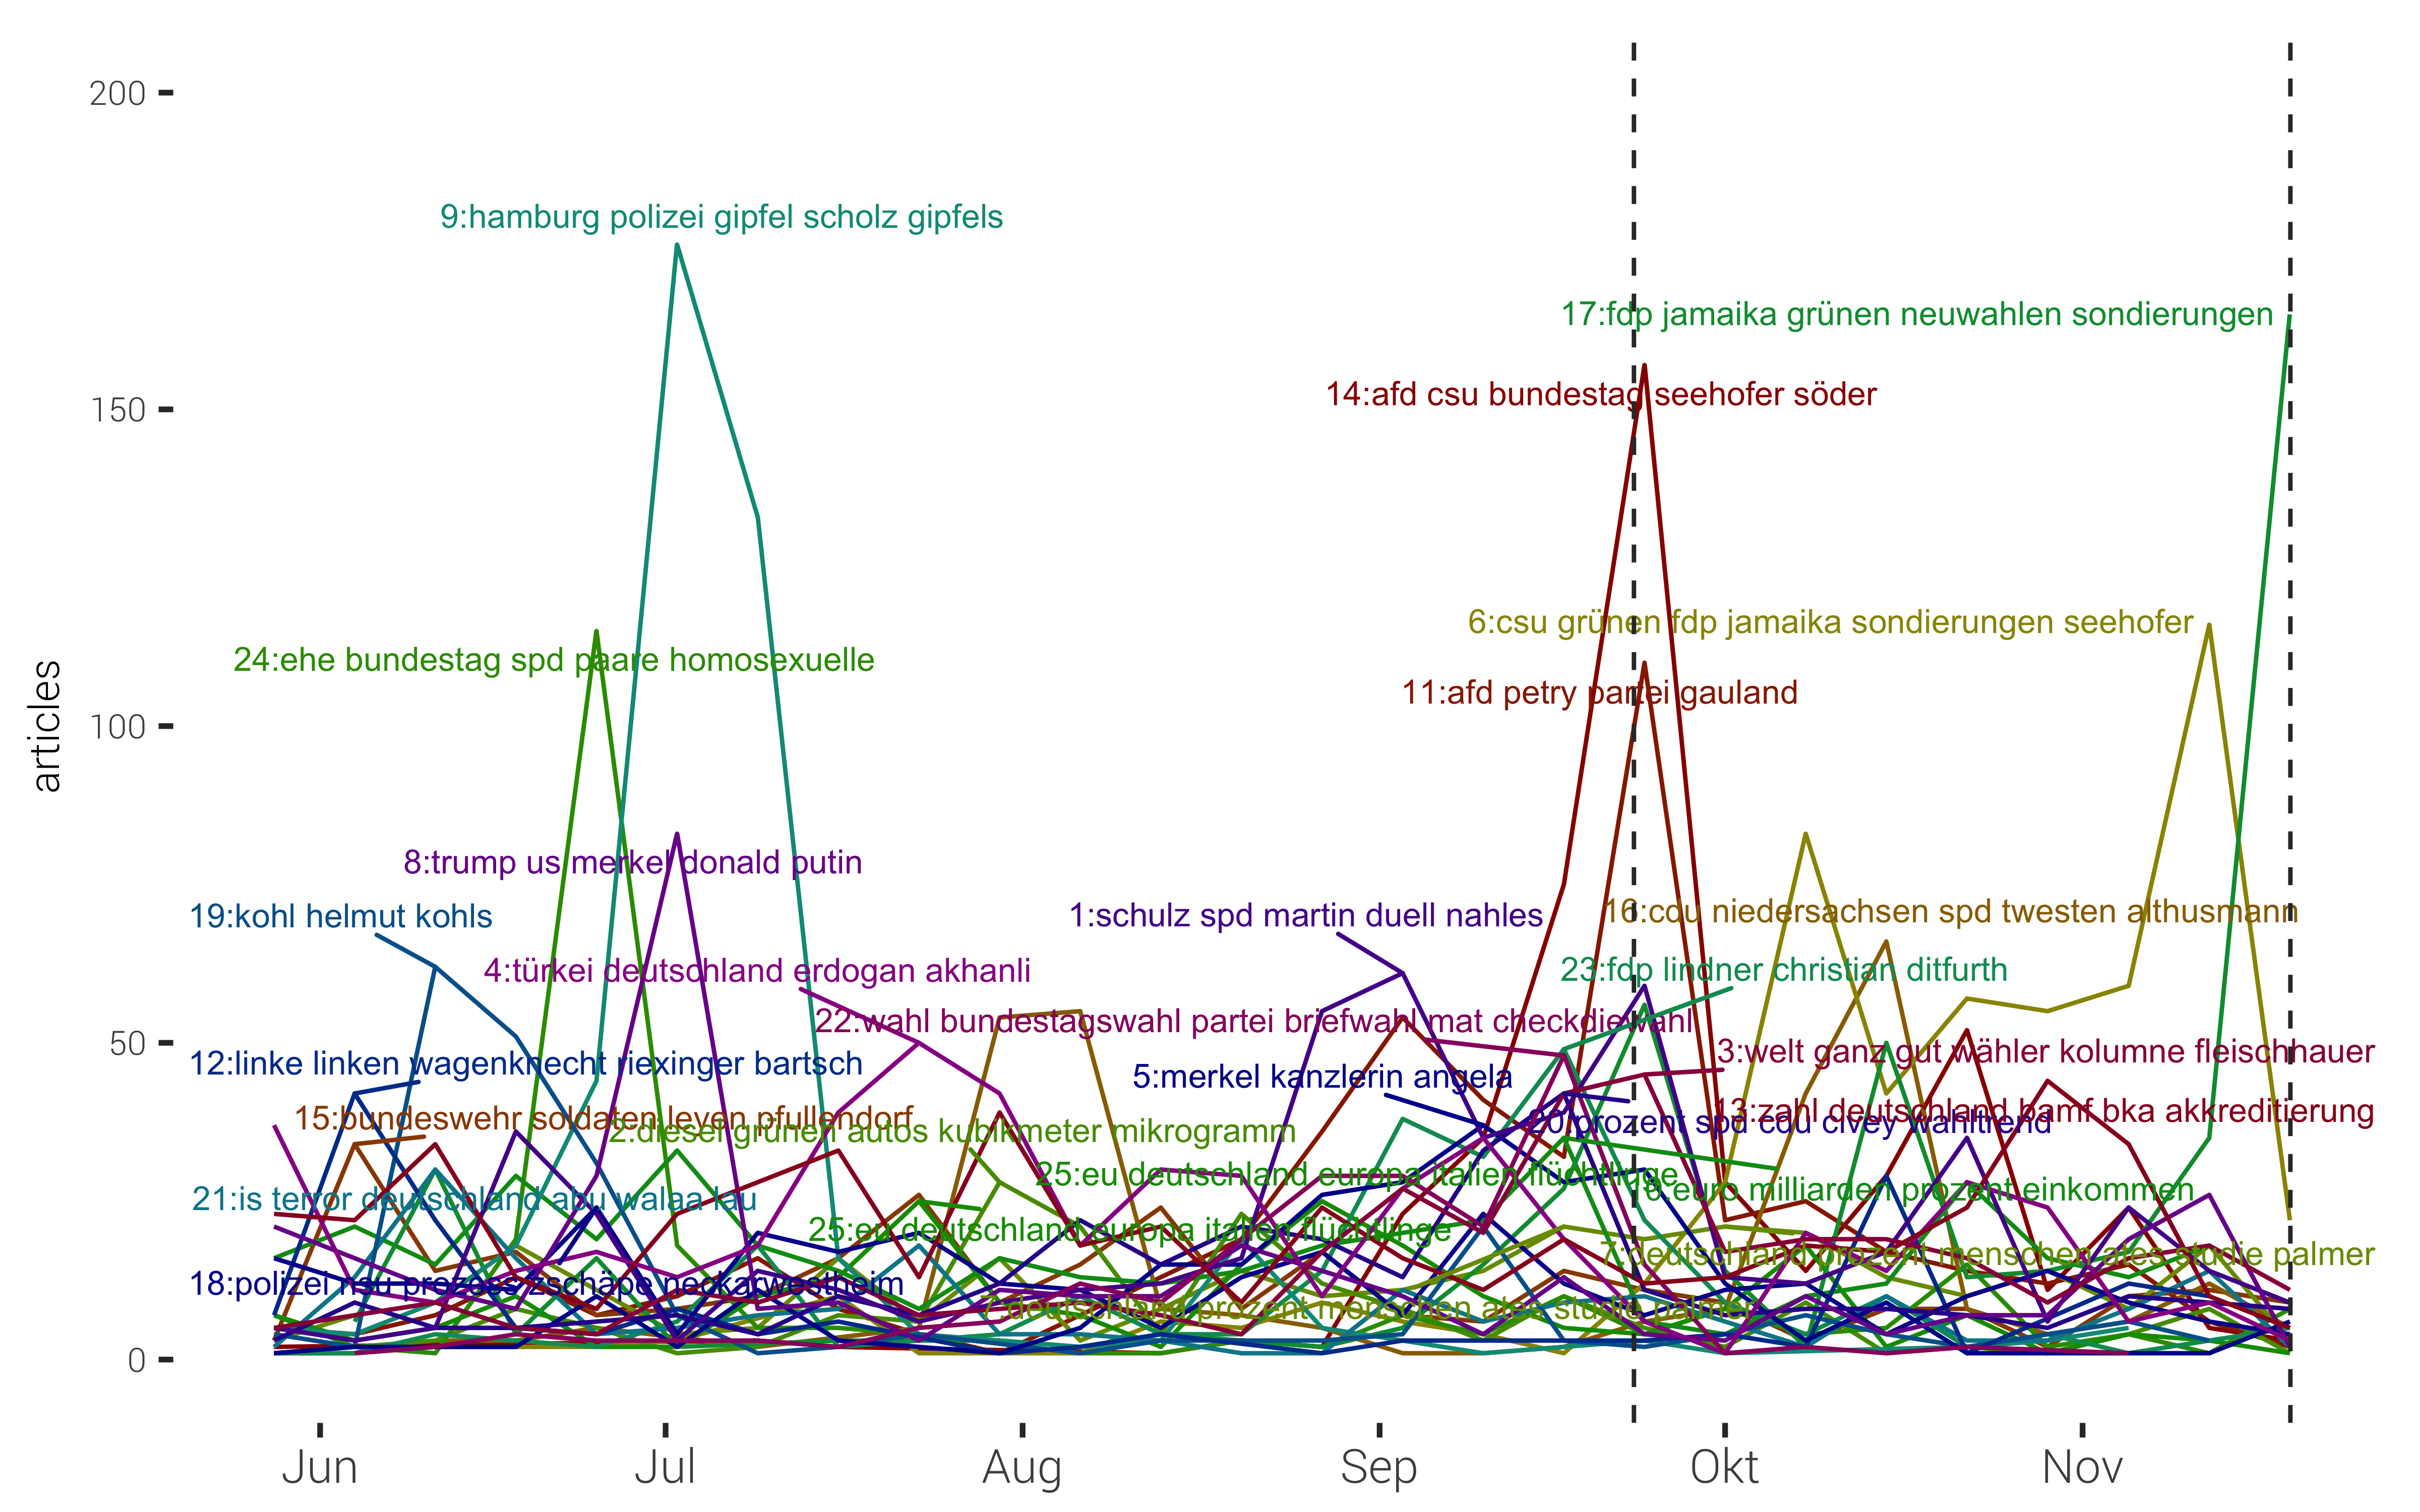
\includegraphics[width=\textwidth,keepaspectratio]{../figs/topic-timeline.png}
			\caption{Topic Timeline}
			\label{fig_topic_timeline}
		\end{subfigure}
	\end{center}
\end{figure}

Model: 

\begin{align*}
	log(FBshares) =\alpha+\beta_{topic}+\beta_{site}+\beta_{textlength}+\epsilon 
\end{align*}


% Table created by stargazer v.5.2 by Marek Hlavac, Harvard University. E-mail: hlavac at fas.harvard.edu
% Date and time: Mi, Dez 06, 2017 - 12:45:38
\begin{table}[!htbp] \centering 
  \caption{} 
  \label{} 
  \begin{adjustbox}{totalheight=\textheight-2\baselineskip}
\begin{tabular}{@{\extracolsep{5pt}}lc} 
\\[-1.8ex]\hline 
\hline \\[-1.8ex] 
 & \multicolumn{1}{c}{\textit{Dependent variable:}} \\ 
\cline{2-2} 
\\[-1.8ex] & fb\_shares\_log \\ 
\hline \\[-1.8ex] 
 topic2 & 0.350$^{*}$ \\ 
  & (0.192) \\ 
  & \\ 
 topic3 & 0.313 \\ 
  & (0.227) \\ 
  & \\ 
 topic4 & 0.533$^{***}$ \\ 
  & (0.159) \\ 
  & \\ 
 topic5 & 0.793$^{***}$ \\ 
  & (0.180) \\ 
  & \\ 
 topic6 & 0.142 \\ 
  & (0.170) \\ 
  & \\ 
 topic7 & $-$0.203 \\ 
  & (0.166) \\ 
  & \\ 
 topic8 & 1.373$^{***}$ \\ 
  & (0.185) \\ 
  & \\ 
 topic9 & 1.040$^{***}$ \\ 
  & (0.153) \\ 
  & \\ 
 topic10 & $-$0.500$^{***}$ \\ 
  & (0.177) \\ 
  & \\ 
 topic11 & $-$0.061 \\ 
  & (0.161) \\ 
  & \\ 
 topic12 & $-$0.565$^{***}$ \\ 
  & (0.187) \\ 
  & \\ 
 topic13 & 0.576$^{***}$ \\ 
  & (0.150) \\ 
  & \\ 
 topic14 & 0.361$^{**}$ \\ 
  & (0.179) \\ 
  & \\ 
 topic15 & $-$0.812$^{***}$ \\ 
  & (0.202) \\ 
  & \\ 
 topic16 & 0.058 \\ 
  & (0.151) \\ 
  & \\ 
 topic17 & 0.311$^{*}$ \\ 
  & (0.186) \\ 
  & \\ 
 topic18 & 0.356$^{*}$ \\ 
  & (0.187) \\ 
  & \\ 
 topic19 & 2.046$^{***}$ \\ 
  & (0.170) \\ 
  & \\ 
 topic20 & 0.0001 \\ 
  & (0.187) \\ 
  & \\ 
 topic21 & 0.934$^{***}$ \\ 
  & (0.161) \\ 
  & \\ 
 topic22 & 0.434$^{**}$ \\ 
  & (0.193) \\ 
  & \\ 
 topic23 & 0.571$^{***}$ \\ 
  & (0.211) \\ 
  & \\ 
 topic24 & 0.975$^{***}$ \\ 
  & (0.170) \\ 
  & \\ 
 topic25 & $-$0.073 \\ 
  & (0.189) \\ 
  & \\ 
 topic26 & 0.258$^{*}$ \\ 
  & (0.152) \\ 
  & \\ 
 topic27 & 0.417 \\ 
  & (0.355) \\ 
  & \\ 
 topic28 & $-$0.067 \\ 
  & (0.194) \\ 
  & \\ 
 siteDIE WELT & 0.389$^{***}$ \\ 
  & (0.112) \\ 
  & \\ 
 siteFOCUS ONLINE & 0.264$^{**}$ \\ 
  & (0.117) \\ 
  & \\ 
 siteSPIEGEL ONLINE & 0.858$^{***}$ \\ 
  & (0.117) \\ 
  & \\ 
 sitestern.de & $-$3.643$^{***}$ \\ 
  & (0.109) \\ 
  & \\ 
 sitetagesschau.de & $-$0.209$^{*}$ \\ 
  & (0.123) \\ 
  & \\ 
 siteZEIT ONLINE & 0.399$^{***}$ \\ 
  & (0.124) \\ 
  & \\ 
 text\_length & 0.0003$^{***}$ \\ 
  & (0.0001) \\ 
  & \\ 
 Constant & 4.594$^{***}$ \\ 
  & (0.148) \\ 
  & \\ 
\hline \\[-1.8ex] 
Observations & 6,743 \\ 
R$^{2}$ & 0.451 \\ 
Adjusted R$^{2}$ & 0.448 \\ 
Residual Std. Error & 2.031 (df = 6708) \\ 
F Statistic & 162.126$^{***}$ (df = 34; 6708) \\ 
\hline 
\hline \\[-1.8ex] 
\textit{Note:}  & \multicolumn{1}{r}{$^{*}$p$<$0.1; $^{**}$p$<$0.05; $^{***}$p$<$0.01} \\ 
\end{tabular}
\end{adjustbox} 
\end{table} 




\end{document}
